\documentclass{VUMIFPSbakalaurinis}
\usepackage{algorithmicx}
\usepackage{algorithm}
\usepackage{algpseudocode}
\usepackage{amsfonts}
\usepackage{amsmath}
\usepackage{array}
\usepackage{bm}
\usepackage{caption}
\usepackage{color}
\usepackage{float}
\usepackage{graphicx}
\usepackage{listings}
\usepackage{longtable}
\usepackage{subfig}
\usepackage{wrapfig}
\usepackage{enumitem}
\usepackage[bottom, multiple]{footmisc}
\usepackage[tableposition=top]{caption}

% --------------------------------------------------------------- %
%                            NUSTATYMAI
% --------------------------------------------------------------- %
\setitemize{noitemsep,topsep=7pt,parsep=0pt,partopsep=7pt}
\setenumerate{noitemsep,topsep=7pt,parsep=0pt,partopsep=7pt}

\newcolumntype{L}[1]{>{\raggedright\let\newline\\\arraybackslash\hspace{0pt}}m{#1}}
\newcolumntype{C}[1]{>{\centering\let\newline\\\arraybackslash\hspace{0pt}}m{#1}}
\newcolumntype{R}[1]{>{\raggedleft\let\newline\\\arraybackslash\hspace{0pt}}m{#1}}

% --------------------------------------------------------------- %
%                            PAGRINDINIS
% --------------------------------------------------------------- %

\bibliography{bibliografija}

% Titulinio aprašas
\university{Vilniaus universitetas}
\faculty{Informatikos institutas}
\department{Programų sistemų katedra}
\papertype{Bakalauro baigiamasis darbas}
\title{Išskirstyto transakcijų žurnalo technologija tiekimo grandinės procesuose}
\titleineng{Distributed Ledger Technology in Supply Chain Processes}
\author{Gediminas Krasauskas}
\supervisor{dr. Evaldas Drąsutis}
\reviewer{partn. doc. Andrius Adamonis}
\date{Vilnius – \the\year}

\begin{document}

\maketitle
% --------------------------------------------------------------- %
%                             PADĖKOS                           
% --------------------------------------------------------------- %

\sectionnonumnocontent{}
\addtocounter{page}{1}
\vspace{7cm}
\begin{center}
    Nuoširdžiai dėkoju savo darbo vadovui Dr. Evaldui Drąsučiui už darbo metu teiktą
    
    konstruktyvią kritiką ir pagalbą.
\end{center}
\sectionnonumnocontent{Santrauka}

Šiame darbe nagrinėjamos IOTA platformos panaudojimo galimybės konkrečiuose tiekimo grandinės procesuose. 
Darbe analizuojama tiekimo grandinių dalykinė sritis, jos sąvoka, struktūra ir šiandieninės problemos.
Aprašyta išskirstyto transakcijų žurnalo technologija, jai keliami reikalavimai tiekimo grandinių kontekste. Išanalizuotos technologijos atmainos, paremtos blokų grandinių ir orientuoto grafo be ciklų principais, pristatytos jų savybės, privalumai ir trūkumai. 
Sukonstruotas pavyzdinis tiekimo grandinės modelis ir diskretūs IOTA platformos taikymo atvejų pavyzdžiai konkrečiuose etapuose, skirti pagrįsti platformos panaudojamumą tiekimo grandinėse. Pateiktos taikymo alternatyvos. 
Darbe pasiūlytos potencialios sistemos svarbiausios užduotys ir veiklos, reikalingos praktinio taikymo įgyvendinimui.

\raktiniaizodziai{Išskirstytas transakcijų žurnalas, blokų grandinė, IOTA, tiekimo grandinė}


% Glaustai aprašomas darbo turinys: pristatoma nagrinėta problema ir padarytos išvados. Santraukos apimtis ne didesnė nei 0,5 puslapio. Santraukų gale nurodomi darbo raktiniai žodžiai. 
% Nurodomi iki 5 svarbiausių temos raktinių žodžių (terminų).
% Vienas terminas gali susidėti iš kelių žodžių.

% Pirmame skyriuje buvo atlikta tiekimo grandinės dalykinės srities analizė: apibrėžta sąvoka, struktūra ir problemoms. Antrajame skyriuje analizuot išskirstyto transakcijų žurnalo technologija, jai keliami reikalavimai iš dalykinės srities pusės, analizuotos technologijos atmainos ir jų savybės, o atmainos palygintos. Remiantis blokų grandinės ir IOTA atmainų savybių palyginimu, pasirinkta viena iš technologijos atmainų, autoriaus vertinimu tinkamesnė taikymui tiekimo grandinėse. Trečiajame skyriuje sumodeliuotas ir pateiktas tiekimo grandinės pavyzdinis atvejis su detaliu paaiškinimu, kiekvienas modelio etapas papildytas IOTA technologinių savybių pritaikymu, konkretūs pavyzdžiai detaliai paaiškinti. Taip pat pristatyti alternatyvūs scenarijai ir taikymo pavyzdžiai, išanalizuotos potencialiai sistemai reikalingos atlikti užduotys, detaliai atvaizduotos užduočių ir veiksmų diagramose.
% --------------------------------------------------------------- %
%                             SUMMARY                           
% --------------------------------------------------------------- %

\sectionnonumnocontent{Summary}

This paper explores the possibilities of using the IOTA platform in specific supply chain processes. The thesis analyzes the subject area of supply chains, its concept, structure and problems. The distributed ledger technology and its requirements in the context of supply chains are described. The types of technology based on the principles of blockchain and directed acyclic graphs were analyzed, their properties, advantages, and disadvantages were presented. An exemplary supply chain model and discrete examples of the application of the IOTA platform at specific stages were designed to support the usability of the platform in supply chains. Application alternatives provided. The thesis suggests the most important tasks and activities of the potential system to implement the practical application.

\keywords{Supply chain, distributed ledger, blockchain, directed acyclic graph, IOTA.}
% --------------------------------------------------------------- %
%                              TURINYS                           
% --------------------------------------------------------------- %

\tableofcontents
\sectionnonum{Įvadas}

XXI a. pasaulį būtų sunku įsivaizduoti be nuolatinio prekių, paslaugų ir informacijos judėjimo. Prekės pastoviai transportuojamos iš vienos vietos į kitą, internetu perduodami milžiniški srautai informacijos, atliekamos transakcijos tarp skirtingų verslo šalių. Tačiau natūraliai pamatyti šiuos procesus vis dėlto nėra toks lengvas uždavinys. Visi šie procesai yra paslėpti po sudėtinga verslo logika, modeliais ir technologijomis. 

Apskritai šie sudėtingi procesai kuria milžinišką pridėtinę vertę, o kartu gerina ir bendrą pasaulinį ekonomikos lygį. Pavyzdžiui, logistika sudaro 7,5\% JAV BVP\footnote{https://www.atkearney.com/transportation-travel/article?/a/2017-state-of-logistics-report-article}, o duomenų srautai 2014 metais prie pasaulinio BVP lygio prisidėjo \$2.8 trln. JAV dolerių \cite{manyika2016digital}. Todėl, siekiant verslo progreso ir konkurencinio pranašumo, šie procesai buvo ir yra optimizuojami bei automatizuojami. Atrodo, kad tai davė savo vaisių. Per pastaruosius dešimtmečius žmonija tapo smarkiai pažangesnė. Prekes transportuoja iki 60 tonų vežantys krovininiai sunkvežimiai \cite{lumsden2004truck} ir per 21 tūkst. TEU standarto konteinerių sugebantys plukdyti krovininiai laivai \cite{halff2019likely}, visuomenės kompiuterinis raštingumas išaugo \cite{van2015internet}, o kartu skaitmenizavosi ir verslas - pradėtos naudoti sudėtingos IT sistemos ir sprendimai.

Pasaulyje esant per 7,5 mlrd. žmonių ir šiam skaičiui vis dar augant\footnote{http://www.worldometers.info/world-population. Tikrinta 2019-02-01}\footnote{\label{note1}https://www.google.com/publicdata/directory. Tikrinta 2019-02-01} bei gerėjant ekonominėms sąlygoms, kartu nenumaldomai auga ir vartojimas\footnote{2012-2017 metais visuotinis BVP padidėjo nuo \$70 iki \$80 trln. JAV dolerių. Duomenys iš https://www.google.com/publicdata/directory. Tikrinta 2019-02-01}, o klientai kelia vis aukštesnius reikalavimus \cite{nilsson2006logistics}. Taigi, norėdamos išlikti konkurencingomis, įmonės varžosi tarpusavyje, naudoja įvairias laiko optimizavimo strategijas, užtikrinančias paslaugų greitį \cite{zacharia2004logistics}, investuoja į vis pažangesnes informacines technologijas. Visa tai tam, kad kad produktas iš gamintojo į pirkėjo rankas patektų kuo kokybiškiau ir optimaliau.

Paprastai šis produkto gyvavimo ciklas, nuo tiekėjo iki pat kliento rankų, yra vadinamas tiekimo grandine. Tiekimo grandinę formaliai galime apibūdinti ir kaip dalyvaujančių organizacijų tinklą, kuris skirtingais procesais ir veiklomis kuria vertę produktų ir paslaugų pavidalu vartotojui \cite{christopher2016logistics}. Tačiau šie apibrėžimai nenusako, kokio masto ir sudėtingumo logistika ir kiti tarpiniai procesai vyrauja tiekimo grandinėse. Vien 2017 metais buvo pasiekta apie 750 milijonų TEU standarto jūrinių konteinerių krova\footnotemark[\ref{note1}], o tais pačiais metais Klaipėdos uosto metinė krova viršijo 43 mln. tonų\footnote{https://sumin.lrv.lt/lt/naujienos/klaipedos-uostas-lyderis-regione. Tikrinta 2019-02-03}. Ir tai tik jūrų krovinių dalis. Remiantis Transparency Market Research duomenimis, iki 2023 metų pajamos visoje logistikos rinkoje turėtų išaugti iki \$15,5 trln. JAV dolerių, o krova iki 92 mlrd. tonų\footnote{https://www.prnewswire.com/news-releases/global-logistics-market-to-reach-us155-trillion-by-2023-research-report-published-by-transparency-market-research-597595561.html. Tikrinta 2019-02-01}.

Šie duomenys nepaprastai svarbūs, nes leidžia suprasti temos aktualumą, t.y. kokią naudą visai žmonijai ir galimybes rinkai gali atverti informacinių technologijų pritaikymas tiekimo grandinėse. Tiesa, įmonės, užsiimančios logistika ir tiekimo grandinių valdymu, jau taiko nemažai informacinių technologijų. Tai programinė įranga ir technologiniai sprendimai, tokie kaip CRM \cite{bharati2015current}, ERP \cite{neubert2018collaboration} ir daugelis kitų. Tačiau visi jie turi savų trūkumų ir nėra tinkami kiekvienai tiekimo grandinei \cite{garg2018supply}.

Bet yra manančių, kad šiandieninėms problemoms spręsti tiekimo grandinėse į pagalbą gali ateiti daiktų internetas \cite{dweekat2017supply} ir iki tol dar plačiai netaikytos paskirstytos didžiaknygės technologijos \cite{abeyratne2016blockchain}. Daiktų internetas padėtų sekti produktų būseną gyvavimo ciklo metu - tai šiuo metu naudojami RFID prietaisai, galintys perduoti informaciją realiu laiku \cite{majeed2017internet}. Tuo tarpu paskirstytų didžiaknygių technologijos plačiau žinomos dėl vienos iš atšakų - blokų grandinės. Tačiau didesnes perspektyvas rodo IOTA technologija \cite{popov2016tangle}, paremta kita paskirstytų didžiaknygių technologijos atšaka - DAG, ir teigianti, jog yra pritaikyta būtent šiai probleminei sričiai . 

IOTA ne tik pasižymi naudingomis paskirstytų didžiaknygių technologijos savybėmis \cite{bramas2018stability}, bet ir leidžia efektyviai išnaudoti daiktų internetą. Tai yra nauja technologija, tačiau jei pavyktų ją sėkmingai pritaikyti praktikoje, ji galėtų tapti inovacija, atnaujinanti procesus, vykstančius kiekvieną dieną ir nuo kurių priklauso mūsų gyvenimo kokybė.

%------------------ TIKSLAS -------------------
Šiuo darbu siekiama įvertinti ir sumodeliuoti galimus pokyčius tradiciniuose tiekimo grandinės modeliuose pradėjus naudoti paskirstytų didžiaknygių technologijas.

%----------------- UŽDAVINIAI -----------------
Šiam tikslui pasiekti keliami tokie uždaviniai:
\begin{itemize}
    \item Apžvelgti tiekimo grandinės dalykinę sritį, jos svarbiausias sąvokas, modelius ir naudojamas technologijas;
    \item Ištirti paskirstytos didžiaknygės technologijų idėją ir atmainas: blokų grandinę ir IOTA, jas palyginti;
    \item Sukonstruoti tiekimo grandinės modelį ir pritaikius IOTA technologiją jį atnaujinti.
\end{itemize}

% Įvade apibrėžiamas tiriamasis objektas akcentuojant neapibrėžtumą, kuris bus išspręstas darbe, aprašomas temos aktualumas, nurodomas darbo tikslas ir uždaviniai, kuriais bus įgyvendinamas tikslas, aptariamos teorinės darbo prielaidos bei metodika, apibūdinami su tema susiję literatūros ar kitokie šaltiniai, temos analizės tvarka, darbo atlikimo aplinkybės, pateikiama žinių apie naudojamus instrumentus (programas ir kt., jei darbe yra eksperimentinė dalis). Darbo įvadas neturi būti dėstymo santrauka. Įvado apimtis 2 -- 4 puslapiai.
% ----------------------------------
\section {Tiekimo grandinė}

Tam, kad galėtume nagrinėti technologijų taikymą tiekimo grandinėse, mums reikia suprasti dalykinę sritį, t.y. kokios yra svarbiausios sąvokos, kokia svarba, mastas, vyraujančios problemos, keliami reikalavimai. Dėl to iš pradžių apžvelgsime šiuos aspektus tolimesniuose poskyriuose.

\subsection{Sąvoka}

Tiksliai ir vienareikšmiškai apibrėžti tiekimo grandinę (angl. \textit{Supply chain}) yra ganėtinai sunkus uždavinys. Apskritai, tai yra pakankamai abstrakti sąvoka, kuri gali keistis nuo konteksto, kuriame yra naudojama ir kuri laikui bėgant nemažai evoliucionavo. Pavyzdžiui, grupė akademikų tiekimo grandinę apibrėžė kaip tris arba daugiau šalis, tiesiogiai susijusias su produktų, paslaugų, finansų ir informacijos judėjimo srautais nuo šaltinio iki kliento \cite{mentzer2001defining}. Tuo tarpu Martin Cristopher tiekimo grandinę įvardijo kaip dalyvaujančių organizacijų tinklą, kuris skirtingais procesais ir veiklomis kuria vertę produktų ir paslaugų pavidalu vartotojui \cite{christopher2016logistics}. 

Taip pat Martin Cristopher savo knygoje diskutuoja, kad tiekimo grandinės sąvokoje žodis „tiekimo“ turėtų būti pakeistas žodžiu „paklausos“ (angl. \textit{Demand}), o žodis „grandinė“ žodžiu „tinklas“ (angl. \textit{Network}). Paklausos sąvoka argumentuojama tuo, kad tiekimo grandinė priklauso ne nuo tiekėjų, o nuo rinkos situacijos, t.y paklausos, na o žodis „tinklas“ labiau atspindėtų realybę, kadangi paprastai yra daugiau nei vienas tiekėjas ir klientas. Tokiu būdu tiekimo grandinės modelis (žr. 1 pav.) taptų panašesnis į paklausos tinklo modelį (žr. 2 pav.).

Nors tinklo modelis yra arčiau realybės, dėl paprastumo ir platesnio sąvokos žinomumo šiame darbe vis dėlto naudosime tiekimo grandinės sąvoką turėdami galvoje tinklo struktūrą. Taigi, pasinaudoję abiem moksliniais šaltiniais, galime suformuluoti išvestinį tiekimo grandinės apibrėžimą - tai organizacijų, procesų, paslaugų, finansų ir informacijos visuma, dalyvaujanti produkto gyvavimo cikle nuo pradinio tiekėjo iki galutinio kliento.

\begin{figure}[H]
    \centering
    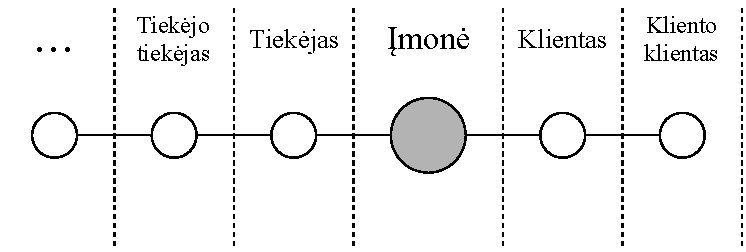
\includegraphics[scale=1]{images/client-supplier-model}
    \caption{Klientų ir tiekėjų sąryšis tiekimo grandinėje}
\end{figure}

Daugelyje mokslinių straipsnių galime aptikti sąvokas „prieš srovę“ (angl. \textit{Upstream}) ir „pasroviui“ (angl. \textit{Downstream}) \cite{croson2005upstream} \cite{frohlich2001arcs} \cite{vachon2006extending}. Tiekimo grandinės kontekste šie žodžiai reiškia įmonės sąryšį su tiekėjais ir klientais. Pavyzdžiui, viską, kas ateina į įmonę iš tiekėjų, paprastai ateina prieš srovę. Tuo tarpu tai, kas išeina iš įmonės pas klientus, atvirkščiai, pasroviui \cite{christopher2016logistics} (žr. 3 pav.). Vėliau įsitikinsime, kad prieš srovę ir pasroviui gali judėti ne tik prekės, bet ir pinigai, informacija ir t.t.

\begin{figure}[H]
    \centering
    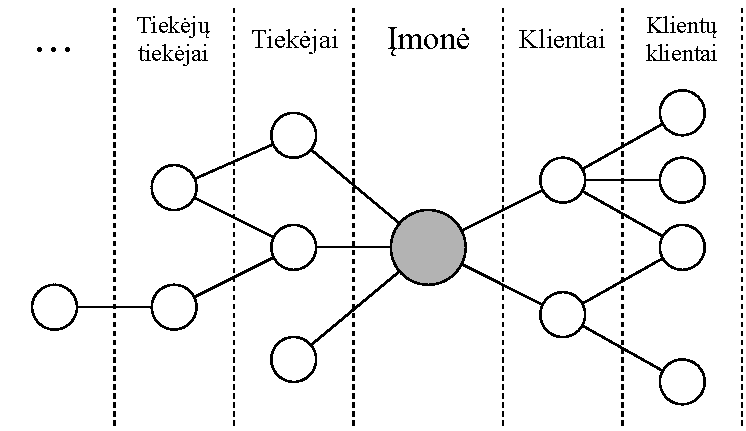
\includegraphics[scale=1]{images/demand-network-model}
    \caption{Paklausos tinklo modelis}
\end{figure}

\begin{figure}[H]
    \centering
    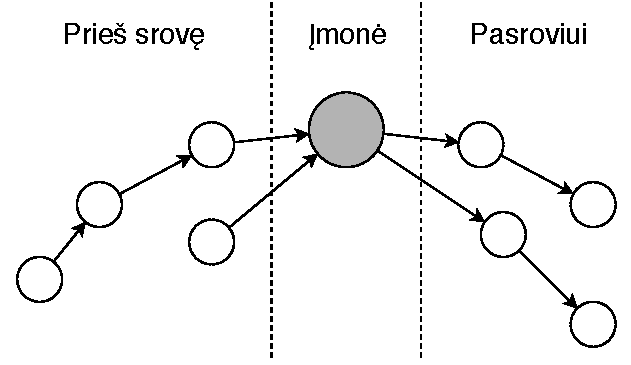
\includegraphics[scale=1]{images/supply-chain-upstream-downstream}
    \caption{Įmonės sąryšiai su tiekėjais ir klientais}
\end{figure}

\subsection{Struktūra}

Nagrinėdami tiekimo grandinės sąvoką sužinojome, kad yra tiekėjų, klientų ir įmonės rolės. Tačiau tai pernelyg abstraktus modelis, kuris nesuteikia gilesnių žinių apie tiekimo grandinės veikimą. Mums svarbu suprasti kas yra tie tiekėjai, ir klientai, kaip šalys bendrauja tarpusavyje, kokios veiklos ir procesai vyksta tiekimo grandinėje. 

Tačiau visa tai labai priklauso ir nuo industrijų, kuriose šios tiekimo grandinės funkcionuoja. Juk procesai ir praktikos, naudojamos maisto pramonėje nebūtinai gali tikti automobilių gamybos industrijoje. Tą patvirtina vien saugumo klausimų skirtumai tarp šių pramonių \cite{marucheck2011product}.

Nagrinėti tikslią realybėje egzistuojančią tiekimo grandinės struktūrą yra sunku ir dėl to, kad įmonės neviešina savo tiekimo grandinės tikslaus gyvavimo ciklo dėl konfidencialumo ir konkurencijos priežasčių. Tačiau moksliniuose ir internetiniuose šaltiniuose\footnote{https://www2.deloitte.com/content/dam/Deloitte/lu/Documents/technology/lu-blockchain-internet-things-supply-chain-traceability.pdf. Tikrinta 2019-02-11} \footnote{https://www.agric.wa.gov.au/newsletters/ovineobserver/ovine-observer-october-2016-76?page=0\%2C2. Tikrinta 2019-02-11} \footnote{https://www.cflex.com/responsibility/social-responsibility/life-cycle-assessment. Tikrinta 2019-02-11} \footnote{https://www.digitalhealth.gov.au/get-started-with-digital-health/what-is-digital-health/supply-chain/life-cycle-of-a-product. Tikrinta 2019-02-11} galime aptikti nemažai pavyzdinių realybę atspindinčių modelių nuo pat žaliavų surinkimo iki pagaminto produkto pristatymo galutiniam pirkėjui \cite{christopher2016logistics} \cite{webber2009building}. Pasinaudoję jais pabandysime sumodeliuoti savo tiekimo grandinę.

[Pabandykime aprašyti įsivaizduojamos įmonės, gaminančios X pavyzdinį tiekimo grandinės scenarijų. Svarbi vieta - pavyzdį naudosiu visame darbe kituose skyriuose jį atnaujinant ir pagerinant su IoT ir DLT. Svarbu sudaryti tokį modelį tokioje industrijoje, kuris leistų atskleisti gerąsias DLT praktikas ir savybes.] 

[Nupasakoti kas vyksta modelyje, svarbiausias vietas paaiškinti]

[Struktūroje pristatyti pinigų, informacijos, reikalavimų ir prekių srautus]

\subsection{Svarba ir industrijos}

\subsection{Šiandieninės problemos}
% --------------------------------------------------------------- %
%           2. IŠSKIRSTYTO TRANSAKCIJŲ ŽURNALO TECHNOLOGIJA
% --------------------------------------------------------------- %

\section {Išskirstyto transakcijų žurnalo technologija} \label{section:dlt}

Kadangi problemos tiekimo grandinėse yra nepašalintos, tai reiškia, kad tradiciniai sprendimai ir technologijos, naudojamos jose, vis dėlto neveikia taip gerai, kaip norėtųsi. Tačiau bet kuriuo atveju, norint vykdyti įmonės apskaitą ir talpinti įrašus ar transakcijas, teks naudotis transakcijų žurnalo (angl. \textit{Ledger}) paslaugomis. O tas, kas teikia transakcijų žurnalo paslaugas, turės įgyvendinti duomenų bazę, kad būtų galima valdyti duomenis.

Tačiau pagrindinė problema kyla dėl to, kad dalyvaujant pirkėjams ir pardavėjams, bei fiksuojant atliekamas transakcijas, yra reikalingas tarpininkas~\cite{gao2018coc}, kuriuo pasitikėtų visos sistema besinaudojančos šalys. Transakcijų žurnalo centralizuotas valdytojas savaime tampa vienvaldžiu tarpininku ir vieninteliu tiesos šaltiniu (angl. \textit{Single source of truth}), o tai suteikia perteklinę įtaką ir galią įrašų manipuliavimui bei kitas potencialias grėsmes~\cite{jiang2017much, shyamasundar2018blockchain}. 

Vienas populiariausių transakcijų žurnalo tarpininko pavyzdžių – bankas. Bankai yra tarpininkai tarp skirtingų šalių, kurios nori atlikti transakcijas tarpusavyje bei laikyti įrašus apie turimą turtą. Bankai sėkmingai gyvuoja dėl to, kad naudotojai, neturėdami kitos išeities ar alternatyvų, pasitiki jais. Tačiau šis pasitikėjimas turi ir savų rizikų. Bankinė institucija potencialiai gali susikompromituoti ir pradėti keisti, ištrinti įrašus savo naudai, taikyti mokesčius už tarpininkavimą ir pasisavinti turtą~\cite{shyamasundar2018blockchain}. Tai yra priežastys, dėl kurių transakcijų žurnalo naudotojai negali iki galo pasikliauti tokiais tarpininkais.

Neseniai vis daugiau susidomėjimo susilaukė išskirstyto transakcijų žurnalo technologija (angl. \textit{Distributed Ledger Technology}), toliau – DLT. Pagrindinė priežastis, kodėl ji atkreipė rinkos, o ypač tiekimo grandinėse ir logistikoje esančių dalyvių dėmesį, yra jos technologinė prasmė. Vienai šaliai priklausantis centralizuotas transakcijų žurnalas pakeičiamas į išskirstytą transakcijų žurnalą, kuris nepriklauso jokiam savininkui, tačiau visi tinklo nariai turi jo kopijas~\cite{shyamasundar2018blockchain}. Tai reiškia pagrindinės problemos sprendimą – pašalintą trečiųjų šalių poreikį~\cite{shyamasundar2018blockchain}. DLT naudojančiai sistemai nebereikia administravimo, o tuo pačiu ir tarpininko mokesčio. Galiausiai užtikrinamas skaidrumas, pašalinant grėsmę, kad tarpininkas piktavališkai išnaudos turimą galią.



% --------------------------------------------------------------- %
%           2.1. IŠSKIRSTYTO TRANSAKCIJŲ ŽURNALO SAVYBĖS
% --------------------------------------------------------------- %

\subsection{Išskirstyto transakcijų žurnalo savybės} \label{subsection:dlt-properties}

Nors pagrindinis DLT išskirtinumas yra tarpininko pašalinimas, jos unikalumas ir ypatybės tuo neapsiriboja. Šią technologiją būtų logiška tirti iš reikalavimų perspektyvos, kurie kyla iš tikimo grandinėse dalyvaujančių suinteresuotų šalių poreikių. Pagrindiniai poreikiai ir DLT savybės nagrinėjamos tolimesniuose poskyriuose.



% --------------------------------------------------------------- %
%                           2.1.1. GREITIS
% --------------------------------------------------------------- %

\subsubsection{Greitis} \label{subsection:dlt-speed}

Šio darbo įžangoje jau buvo pabrėžta, kokio dydžio ir masto informacijos srautai bei transakcijų kiekiai vyrauja tiekimo grandinėse. Naudojamas transakcijų žurnalas turėtų būti labai greitas, t.y. gebėti apdoroti šimtus tūkstančių įrašų per labai trumpą laiko tarpą, tiek juos rašant, tiek nuskaitant. Šis rodiklis gali būti matuojamas transakcijomis per sekundę (angl. \textit{Transactions per second}), toliau – TPS, nusakančiu kaip greitai įrašas atsiduria transakcijų žurnale. Natūralu, kad kuo ilgesnis laukimo laikas, tuo daugiau nuostolių gali patirti transakcijų žurnalo naudotojai. Ateityje šie apkrovos rodikliai turėtų nenumaldomai augti dėl vis labiau taikomo daiktų interneto~\cite{kaur2018edge}. 

Vienas iš įrašų kūrimo pavyzdžių – radijo dažnio identifikavimo (angl. \textit{Radio Frequency Identification}) technologijos, toliau – RFID. Jeigu kiekviename konteineryje, maisto plantacijose, fabrikuose ir t.t. būtų naudojamas vienas ar keli RFID davikliai, kurie paneštų savo būseną numatytu laiko periodu, tai lemtų milijardinius aktyvių tinkle esančių dalyvių kiekius per parą pasauliniu mastu.

Be to, visi šie duomenys turėtų būti saugomi ilgą laiką. Įmonėms gali prireikti prieš kelis metus atliktų transakcijų, vykdytų operacijų arba individualių RFID daviklių istorinių duomenų. Svarbus ir duomenų atsekamumas, kad būtų galima stebėti krovinių kelionę ir būseną, net jei šie duomenys buvo kaupiami tam tikrose vietose neturint interneto ryšio. Greitas ir stabilus visų šių duomenų valdymas tampa sudėtingu IT infrastruktūriniu uždaviniu.

Nors duomenų apdorojimo greitis yra ko gero svarbiausias kriterijus, į kurį turi atsižvelgti technologijos, DLT iš savęs nepateikia sprendimo greičio klausimui spręsti. Tai – konkrečios DLT architektūros klausimas, nuo kurios ir priklauso, kokie sprendimai bus įgyvendinami, norint išpildyti greičio reikalavimus.

Tradicinės transakcijų žurnalų sistemos iš esmės yra išsprendusios greičio klausimus ir gali apdoroti tūkstančius transakcijų per sekundę\footnote{Mokėjimų platformos, tokios kaip PayPal, vykdo apie 136 TPS, o Visa nuo 2 tūkst. TPS iki 56 tūkst. TPS~\cite{herrera2016privacy}.} ar net milijonus transakcijų per sekundę\footnote{Šiuos rodiklius demonstruoja duomenų bazių valdymo sistemos, tokios kaip Oracle: \href{https://blogs.oracle.com/timesten/scaling-sql-to-millions-of-transactions-per-second-with-a-single-database}{https://blogs.oracle.com/ timesten/scaling-sql-to-millions-of-transactions-per-second-with-a-single-database} [žiūrėta 2019-05-14].}. Tačiau naudojant DLT, dėl savo subtilybių ir specifikos, greičio problemos atsiranda kitu pavidalu. Kiekvieno įrašo padarymas yra konsensuso algoritmo (angl. \textit{Consensus Algorithm}) dalis. Konsensuso algoritmas – tai protokolas, kuris pasirūpina, kad visi tinklo nariai sinchronizuotųsi tarpusavyje ir prieitų bendrą sutarimą įvertinant, kurios transakcijos yra tinkamos, kad jas būtų galima pridėti į transakcijų žurnalą~\cite{cachin2017blockchain}. 



% --------------------------------------------------------------- %
%                     2.1.2. DUOMENŲ NEKINTAMUMAS
% --------------------------------------------------------------- %

\subsubsection{Duomenų nekintamumas} \label{subsection:dlt-immutability}

Tiekimo grandinėse ypatingai svarbu, kad įrašai nebūtų padirbinėjami arba sunaikinami be žinios ar nepageidaujamo įsikišimo. Šiuo metu vyraujant centralizuotoms duomenų bazėms, administratoriai gali manipuliuoti duomenimis, o fizinės duomenų saugyklos, įvykus nenumatytiems incidentams, gali būti pažeistos nepataisomai.

DLT siūlo decentralizuoto transakcijų žurnalo architektūrą (žr.~\ref{img:5} pav.), kurio veikimui nereikia jokios centralizuotos duomenų saugyklos ar administravimo~\cite{yu2018virtualization}. Transakcijų žurnalas tampa paskirstytas visame tinkle ir, naudojant konsensuso algoritmą, visi autorizuoti pakeitimai bet kurio vartotojo transakcijų žurnalo kopijoje atsispindi visų tinkle esančių vartotojų kopijose~\cite{puthal2018blockchain}. Taip yra todėl, kad tinklo nariai, norėdami skaityti arba rašyti informaciją, kreipiasi ne į centrinę duomenų saugyklą, o į tinklą, t.y. tinkle dalyvaujančius narius ir jų duomenis.

\begin{figure}[H]
    \centering
    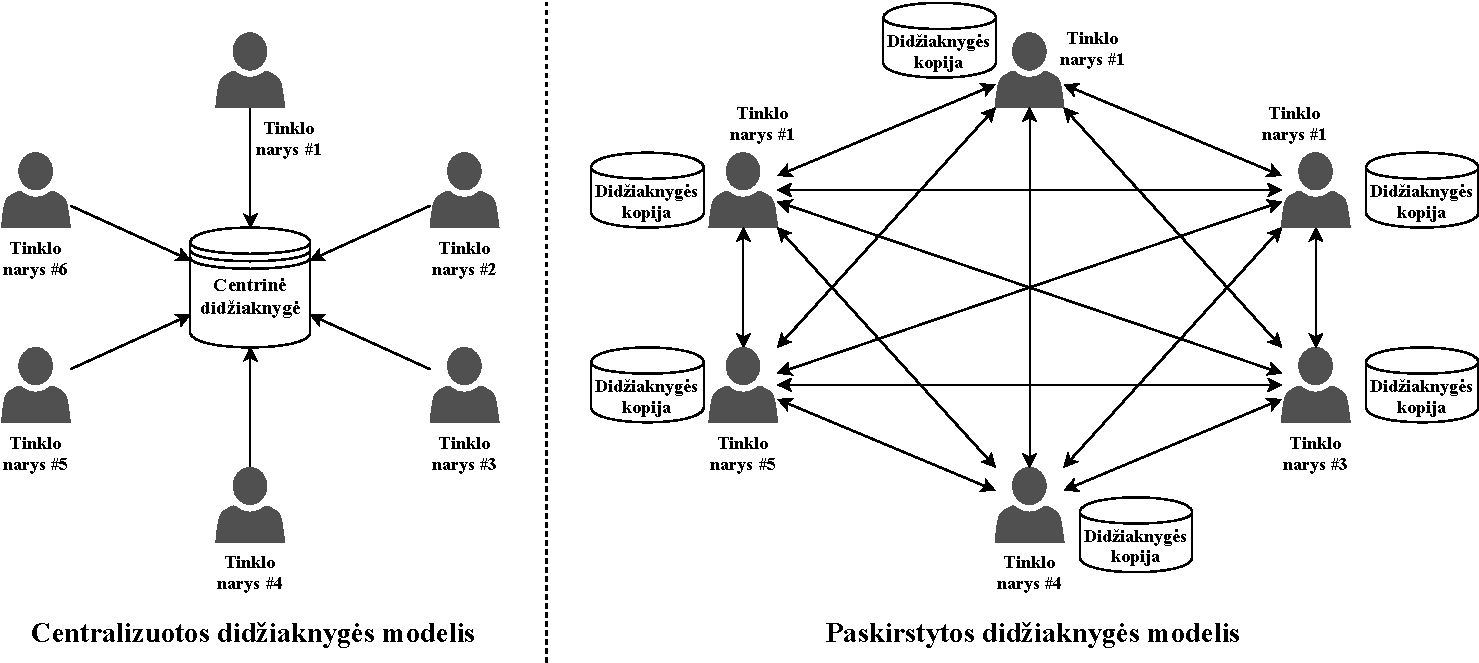
\includegraphics[scale=0.63]{images/ledger-model-types}
    \caption{Transakcijų žurnalo centralizuoto ir išskirstyto tipų modeliai}
    \label{img:5}
\end{figure}

Iš to kyla viena svarbiausių DLT savybių: tai, kas įrašyta į išskirstytą transakcijų žurnalą, negali būti pakeista arba ištrinta – šitaip yra pasiekiamas duomenų nekintamumas (angl. \textit{Data Immutability})~\cite{xu2017dl}. Tokiu atveju visi duomenys tampa apsaugoti nuo potencialaus duomenų padirbinėjimo. O tai leidžia matyti visą unikalią istorinę informaciją. Pavyzdžiui, transportuojant prekes iš taško A į tašką B ir fiksuojant krovinio vietą laike, galime matyti visą jo kelionės istorinę informaciją ir pasitikėti išskirstytu transakcijų žurnalu, jog tie duomenys yra autentiški. 

Tą užtikrina jau minėtas konsensuso algoritmas, apsaugantis duomenis nuo piktavalių naudotojų. Tačiau ši savybė tam tikrais atvejais gali būti tuo pačiu ir trūkumas. Pavyzdžiui, kai naudojame informaciją, galinčią dažnai kisti. Pasikeitus kliento mobilaus telefono numeriui, atnaujinti esamo duomenų įrašo negalėtume ir tektų kurti naują įrašą apie atsinaujinusius kliento duomenis.



% --------------------------------------------------------------- %
%                       2.1.3. DUOMENŲ SAUGUMAS
% --------------------------------------------------------------- %

\subsubsection{Duomenų saugumas} \label{subsection:dlt-security}

Svarbu, kad privatūs ir jautrūs duomenys, kuriais disponuoja įmonės, būtų apsaugoti, o prieigą prie jų turėtų tik tie, kam duomenys priklauso arba turi leidimą juos valdyti. Tai tapo dar svarbesniu veiksniu 2018 metais įsigaliojus GDPR reglamentui~\cite{ferrari2018eu}. Jeigu įmonės paviešintų jautrią informaciją, ji patirtų milžiniškus piniginius nuostolius dėl baudų, o nutekinta įmonei svarbia informacija pasinaudotų jos konkurentai.

Didelė dalis populiariausių DLT yra viešos, nereikalaujančios prieigos teisių (angl. \textit{Permissionless Ledger}), t.y. visi vartotojai turi prieigą prie transakcijų žurnalo~\cite{olnes2017blockchain}. Šitaip viešai matoma kas ir kokią informaciją įrašo į paskirstytą žurnalą, o tuo pačiu bet kas gali kurti naujus įrašus. Tačiau galimos ir papildomos DLT konfigūracijos. Pavyzdžiui, galima sukurti tokį privatų išskirstytą transakcijų žurnalą (angl. \textit{Permissioned Ledger}), kuriame duomenis skaityti bei rašyti galėtų tik prieigos teisę turinčios šalys~\cite{backlund2016technical}. Tai yra naudinga, jeigu dvi ar daugiau įmonių yra verslo partnerės ir nori dalintis bendra informacija ar atlikti transakcijas tarpusavyje, tačiau jos nenorėtų, kad bet kas kitas už šio rato ribų apie tai žinotų. 

Vis dėlto, duomenis apsaugoti galima ir kitais būdais. Pavyzdžiui, naudojant kriptografijos metodus, tokius kaip privatų ir viešą raktą~\cite{zyskind2015decentralizing}, galime užšifruoti duomenis ir į išskirstytą transakcijų žurnalą įrašyti tik tam tikrą maišos reikšmę (angl. \textit{Hash value}). Tiesa, visi tinklo nariai matys kas šiuos duomenis patalpino, tačiau niekas negalės žinoti duomenų turinio, išskyrus šalis, turinčias privatų raktą. Tai leidžia talpinti jautrią informaciją į viešą DLT ir jaustis saugiai, nes peržiūrėti jos originalų formatą be leidimo, t.y. privataus rakto, negali niekas.



% --------------------------------------------------------------- %
%           2.2. IŠSKIRSTYTO TRANSAKCIJŲ ŽURNALO ATMAINOS
% --------------------------------------------------------------- %

\subsection{Išskirstyto transakcijų žurnalo atmainos} \label{subsection:dlt-types}

Yra du pagrindiniai DLT tipai. Tai blokų grandinės (angl. \textit{Blockchain}) ir orientuoto grafo be ciklų (angl. \textit{Directed Acyclic Graph}), toliau – DAG struktūrą turintys DLT, kurie bus analizuojami tolimesniuose poskyriuose.



% --------------------------------------------------------------- %
%                       2.2.1. BLOKŲ GRANDINĖ
% --------------------------------------------------------------- %

\subsubsection{Blokų grandinė} \label{subsection:blockchain}

Šiuo metu yra daug blokų grandinių projektų, tačiau populiariausiomis ir stabiliausiomis išlieka dvi – Bitcoin ir Ethereum\footnote{Duomenys paimti iš: \href{https://coinmarketcap.com}{https://coinmarketcap.com} [žiūrėta 2019-05-14].}. Šios blokų grandinės veikia tokiu principu: blokų duomenų struktūros, kuriose saugoma informacija, t.y. transakcijos bei kitos blokų grandinės veikimui reikalingos reikšmės, yra sujungtos tarpusavyje nuosekliai į vieną ilgą ir nenutrūkstamą seką (žr.~\ref{img:6} pav.)\footnote{Paveikslėlyje pavaizduota architektūra yra prototipinė autoriaus sukurta blokų grandinė. Realybėje egzistuojančių blokų grandinių architektūros yra kur kas sudėtingesnės.}. Vienintelis būdas sukurti naujus įrašus – surinkti juos į naują bloką ir prijungti jį prie paskutinio grandinėje esančio bloko.

\begin{figure}[H]
    \centering
    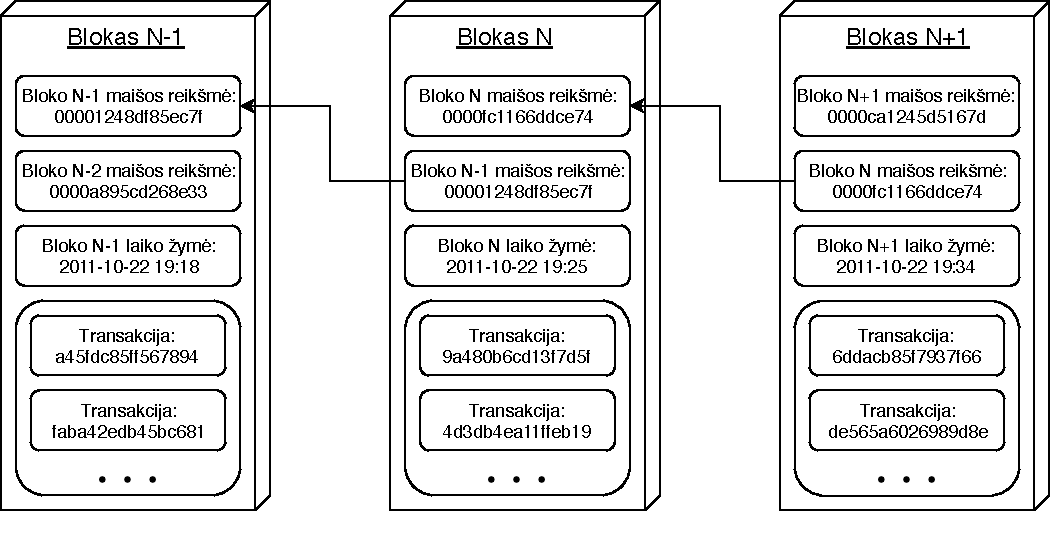
\includegraphics[scale=0.80]{images/block-chain-architecture}
    \caption{Blokų grandinės architektūrinis modelis}
    \label{img:6}
\end{figure}



% --------------------------------------------------------------- %
%          2.2.1.1. BLOKŲ GRANDINĖS DUOMENŲ NEKINTAMUMAS
% --------------------------------------------------------------- %

\subsubsubsection{Blokų grandinės duomenų nekintamumas} \label{subsection:blockchain-immutability}

Jeigu bandytume pridėti bloką grandinės viduryje, ši išsišakotų į 2 atskiras šakas. Čia svarbią reikšmę turi konsensuso algoritmas. Konsensuso algoritmas turi apsaugoti blokų grandinę nuo grandinės išsišakojimų, blokų ištrynimo, keitimo, dvigubo išleidimo problemos (angl. \textit{Double-spending problem}) bei kitokių taisyklių pažeidimų ar spragų, kuriomis norėtų pasinaudoti kenkėjai tinkle~\cite{baliga2017understanding}. Kitaip – garantuoti duomenų nekintamumą ir vienareikšmiškumą.

Vienas iš tokių konsensuso algoritmo atmainų, kurį naudoja Bitcoin ir Ethereum, yra atlikto darbo (angl. \textit{Proof of Work}) konsensuso algoritmas, toliau – PoW~\cite{gervais2016security}. Kaskart norint pridėti bloką, reikia atlikti darbą, kuris reikalauja kompiuterinių skaičiavimų galios, laiko ir energijos išteklių. Blokų grandinėje kuriant naujus blokus tam tikrais atvejais atsiranda išsišakojimų. Tai įvyksta tada, jeigu du ar daugiau blokų iškasami beveik tuo pačiu metu~\cite{zheng2017overview}. Atsiradus tokiems išsišakojimams, tinklas pasirenka ilgiausią atšaką, t.y. tokią, kuri turi daugiausiai blokų~\cite{zheng2017overview}. 

Tačiau išsišakojimus galima kurti ir savanaudiškais tikslais. Tinklo kenkėjas, norintis pakeisti transakciją viename iš blokų, sukurs grandinės išsišakojimą, turintį savyje pakeistos transakcijos versiją. Tačiau tam, kad tinklas pripažintų pakeistą transakciją grandinėje, t.y. naują grandinės išsišakojimą, kenkėjas turės atlikti darbą, kurį padarė visas tinklas nuo išsišakojimo pradžios iki einamojo momento~\cite{nakamoto2008bitcoin}. Be to, atlikti PoW darbą reikės gerokai sparčiau nei visi kiti tinklo nariai kartu sudėjus, kad kenkėjas ne tik pasivytų visą tinklą grandinės ilgiu, bet ir jį aplenktų. Visa tai tam, kad kenkėjo sukurtas grandinės išsišakojimas taptų ilgesnis už pagrindinę grandį\footnote{Šis scenarijus dar yra vadinamas 51 procento ataka (angl. \textit{51\% Attack)}~\cite{baliga2017understanding}.}~\cite{nakamoto2008bitcoin}. Tik tokiu atveju piktybinę grandį tinklas priimtų kaip teisingą (žr.~\ref{img:7} pav.).

Šiuo metu tiek Bitcoin, tiek Ethereum toks scenarijus yra mažai tikėtinas, nes naujus blokus sukuria didelis kiekis kasėjų (angl. \textit{Miners}), kuriems PoW suteikia stimulą (angl. \textit{Incentive}) kasti, t.y. kurti naujus blokus. Tą lemia PoW skatinimo sistema: už kiekvieną iškastą bloką yra skiriamas apdovanojimas – kriptovaliuta (angl. \textit{Cryptocurrency})~\cite{nakamoto2008bitcoin}. Taigi, tinklo kenkėjui beveik nėra šansų pakreipti konsensuso algoritmo savo naudai – to daryti tiesiog neapsimoka ir beveik neįmanoma techniškai. Šitaip užtikrinamas vienas iš reikalavimų – duomenų nekintamumas ir vienareikšmiškumas.

\begin{figure}[H]
    \centering
    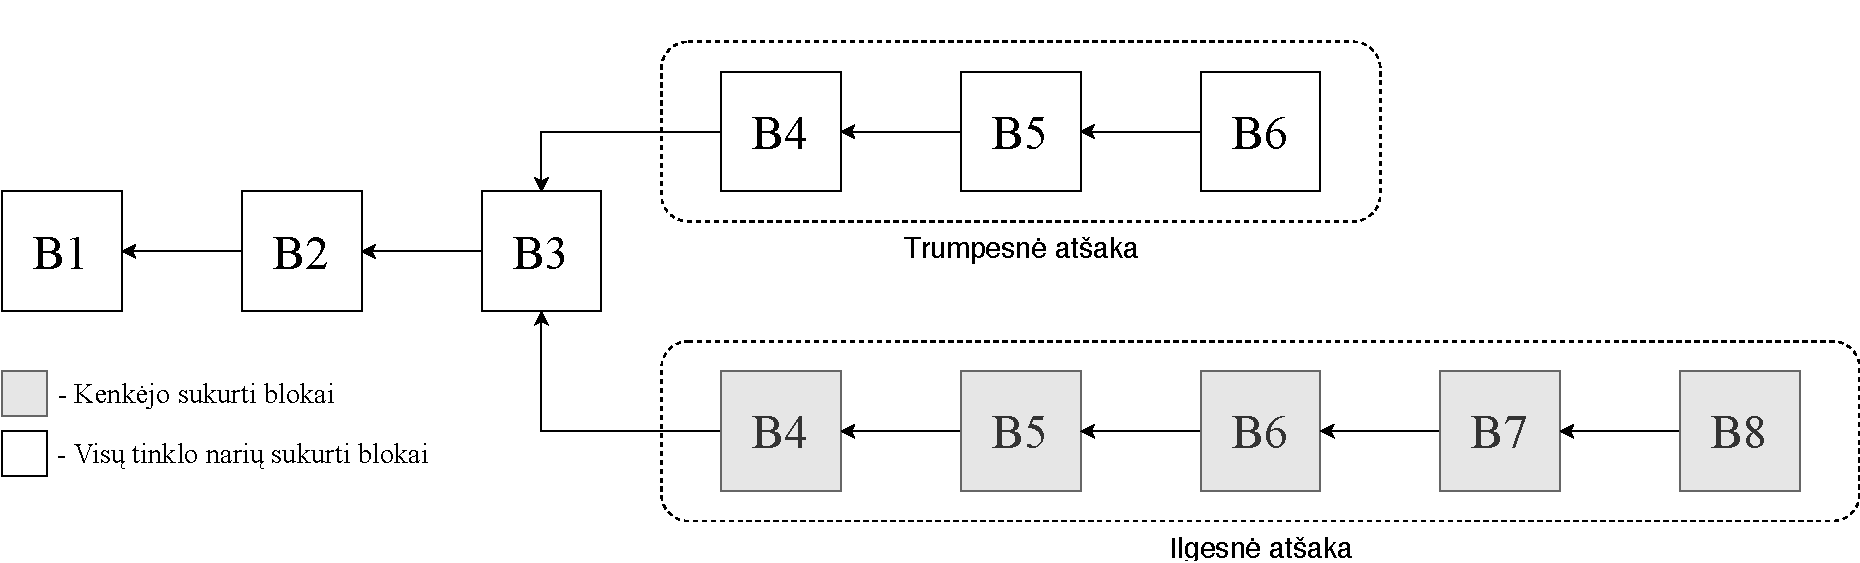
\includegraphics[scale=0.45]{images/blockchain-branches}
    \caption{Blokų grandinės šakos~\cite{zheng2017overview}}
    \label{img:7}
\end{figure}



% --------------------------------------------------------------- %
%               2.2.1.2. BLOKŲ GRANDINĖS PRALAIDUMAS
% --------------------------------------------------------------- %

\subsubsubsection{Blokų grandinės pralaidumas} \label{subsection:blockchain-throughput}

Blokų grandinės pralaidumas (angl. \textit{Throughput}) priklauso nuo daugelio faktorių. Visi šie faktoriai yra susiję su transakcijų gyvavimo ciklu. Bitcoin atveju transakcijų gyvavimo ciklas veikia tokiu principu~\cite{nakamoto2008bitcoin}:
\begin{enumerate}
    \item Visų pirma, kiekvienas narys, sukurdamas transakciją, ją viešai paskelbia kitiems tinklo nariams tam, kad transakcija būtų įtraukta į bloką. 
    \item Bloko kasėjas surenka dalį arba visas viešai paskelbtas transakcijas į bloką ir atlieka darbą pagal PoW konsensuso algoritmą.
    \item Apskaičiavęs darbo rezultatą kasėjas paskelbia naujai sukurtą bloką visiems tinklo nariams viešai. 
    \item Jeigu kiti tinklo nariai pasitiki bloke esančių transakcijų tinkamumu, blokas galiausiai prijungiamas prie visos grandinės pabaigos ir tinklas nuosekliai jungia naujus blokus prie šio bloko. 
\end{enumerate}

Tačiau tuo bloko gyvavimo ciklas nesibaigia. Jeigu blokas prijungiamas prie grandinės, dar nereiškia, kad jis laikomas patvirtintu. Tam, kad blokas būtų laikomas saugiai patvirtintu, o kartu su juo ir transakcijos jame, prie šio bloko nuosekliai dar turi būti prijungtas tam tikras kiekis blokų. 

Taip pat yra tikimybė, kad transakcija nebus patvirtinta, jeigu blokų kasėjai jos neįtrauks į blokus. Blokų kasėjai renkasi transakcijas pagal tai, kokią jie naudą gaus pridėdami jas į bloką. Ši nauda matuojama transakcijos mokesčiu (angl. \textit{Transaction fee}), kurį nurodo transakcijos kūrėjas. Taigi, gali atsitikti taip, kad, transakcijos kūrėjas pasiūlys per mažą kainą už savo transakcijos įtraukimą į bloką ir ji bus patvirtinta gerokai vėliau arba netgi niekada\footnote{Scenarijus tikėtinas, jeigu transakcijų, laukiančių patvirtinimo, yra daugiau negu telpa viename bloke.}.

Taigi matome, kad transakcijų greitis priklauso nuo šių pagrindinių priežasčių: 
\begin{itemize}
    \item Mokesčio dydžio, kuris lemia, ar kasėjai bus linkę įtraukti transakciją į blokus ir kaip greitai ji bus įtraukta.
    \item Kiek blokas gali talpinti savyje transakcijų, arba kitaip bloko dydis baitais.
    \item Kiek laiko trunka bloko sukūrimas, kitaip – per kiek laiko atliekamas PoW skaičiavimas.
    \item Kiek reikalinga tolimesnių blokų, kad blokas būtų laikomas saugiai patvirtintu.
\end{itemize} 

Žemiau pateikiama lentelė (žr.~\ref{tab:1} lentelę) su Bitcoin ir Ethereum platformų rodiklių palyginimais\footnote{Autorius nepateikia vidutinės transakcijos mokesčio kainos, nes kriptovaliutų kaina ir transakcijos mokestis rinkoje yra labai nepastovūs. Ethereum: \href{https://ethgasstation.info}{https://ethgasstation.info}, Bitcoin: \href{https://bitcoinfees.info}{https://bitcoinfees.info} [žiūrėta 2019-05-17].}. Iš joje esančių duomenų seka maksimalus TPS greitis.

\begin{longtable}{|L{4cm}|L{5,3cm}|L{5,5cm}|}
\caption{Bitcoin ir Ethereum rodiklių palyginimas}
\label{tab:1}
\endfirsthead
\endhead
\hline
\textbf{Palyginimo kriterijus} & \multicolumn{1}{c|}{\textbf{Bitcoin}} & \multicolumn{1}{c|}{\textbf{Ethereum}} \\ \hline
\textbf{Transakcijų kiekis bloke} & Apie 4000~\cite{zhu2016interactive} & 380 limitas\footnote{Bloko GAS limitas – 8 mln.~\cite{hu2018hierarchical}, o vienos transakcijos minimalus GAS limitas – 21 tūkst.~\cite{xu2017taxonomy}. Todėl 8000000 / 21000 = 380.} \\ \hline
\textbf{Bloko iškasimo laikas} & 10 min.~\cite{macdonald2017blockchain} & 10-20 sekundžių~\cite{gervais2016security} \\ \hline
\textbf{Patvirtinimo blokų skaičius} & 6~\cite{xu2017taxonomy} & 12~\cite{xu2017taxonomy} \\ \hline
\textbf{Saugaus patvirtinimo laikas} & 1 valanda~\cite{xu2017taxonomy} & 3 minutės~\cite{xu2017taxonomy}  \\ \hline
\textbf{TPS limitas} & 7 TPS~\cite{macdonald2017blockchain} & 25 TPS~\cite{bocek2018smart} \\ \hline
\end{longtable}



% --------------------------------------------------------------- %
%                 2.2.1.3. BLOKŲ GRANDINIŲ TRŪKUMAI
% --------------------------------------------------------------- %

\subsubsubsection{Blokų grandinių trūkumai} \label{subsection:blockchain-drawbacks}

1 lentelėje pateikti duomenys atskleidžia blokų grandinių trūkumus. Žinant tiekimo grandinių ir logistikos mastus, šiuo metu šios platformos turėtų rimtų sunkumų siekiant patenkinti rinkos poreikius dėl esamų technologinių suvaržymų: 
\begin{itemize}
    \item TPS limitai. Būtų sunku įsivaizduoti didelių sistemų funkcionavimą bent vienoje iš šių platformų, nes jos negalėtų susitvarkyti su milijoniniu transakcijų krūviu. Logistikoje yra įprasta, kad vien individualios siuntos kelionės gyvavimo cikle dažnai pasikeičiant savininkams, yra atliekama keletas ar net dešimtys transakcijų.
    \item Patvirtinimo laukimo laikas. Tiekimo grandinėse laikas yra svarbus ir kainuoja pinigus. Laukti kelioliką minučių ar net valandą, kol transakcija bus patvirtinta, stabdytų įprastą tiekimo grandinės tėkmę ir atneštų didelių nuostolių. Be to, naudojant blokų grandines egzistuoja tikimybė, kad transakcija taip ir nebus įtraukta į blokų grandinę ir ją teks atlikti iš naujo.
    \item Mokesčiai už atliekamas transakcijas tikriausiai yra vienas iš labiausiai atgrasančių suvaržymų. Tikėtina, kad tam tikrais atvejais mokesčiai už transakcijas gali būti aukštesni už transportuojamų prekių kainą.
\end{itemize} 

Tam tikros blokų grandinės yra įgyvendinusios išmaniųjų kontraktų (angl. \textit{Smart contracts}) funkcionalumą, kuris praturtina technologijos potencialą. Išmanusis kontraktas – programinis kodas, kuris vykdo komandas pagal prieš tai aprašytas taisykles~\cite{buterin2013ethereum}.

Ethereum išmanieji kontraktai įgalina automatizuotus kriptovaliutų pervedimus pagal programinį kodą, remiantis užprogramuotais scenarijais. Tačiau jų realizavimas praktikoje kol kas atrodo neefektyvus. Visi tinklo nariai, norintys patikrinti bloko validumą, turintį savyje transakciją, kuri inicijuoja išmaniojo kontrakto vykdymą, turi vykdyti tą patį išmaniojo kontrakto kodą~\cite{buterin2013ethereum}. Dėl šios priežasties vienos decentralizuotos programėlės (angl. \textit{Decentralized Application}), toliau - DApp, išpopuliarėjimas apkrovė ir smarkiai sulėtino Ethereum tinklą\footnote{Informacija paimta iš: \href{https://cryptovest.com/news/ethereum-loses-to-cryptokitties-network-remains-slow}{https://cryptovest.com/news/ethereum-loses-to-cryptokitties-network-remains-slow} [žiūrėta 2019-05-17].}.\pagebreak



% --------------------------------------------------------------- %
%               2.2.2. ORIENTUOTAS GRAFAS BE CIKLŲ
% --------------------------------------------------------------- %

\subsubsection{Orientuotas grafas be ciklų} \label{subsection:dag}

Šiuo metu egzistuoja gerokai mažiau DAG principu paremtų projektų, negu jų yra blokų grandinių aplinkoje. Tačiau vienas iš įdomiausių ir daugiausiai žadančių – IOTA platforma. 



% --------------------------------------------------------------- %
%                   2.2.2.1. IOTA VEIKIMO POBŪDIS
% --------------------------------------------------------------- %

\subsubsubsection{IOTA veikimo pobūdis} \label{subsection:dag-principals}

Vietoje blokų grandinės ir joje kasamų blokų su transakcijomis, IOTA įgyvendino DAG struktūrą turinčią išskirstytą transakcijų žurnalą, vadinamą raizginiu (angl. \textit{Tangle}) (žr.~\ref{img:8} pav.). Modelyje vaidmenį atlieka 3 elementai:
\begin{itemize}
    \item Patvirtinta transakcija. Tai tokia transakcija, kurią patvirtina bent viena kita transakcija.
    \item Nepatvirtinta transakcija. Jos dar vadinamos raizginio viršūnėmis (angl. \textit{Tips}). Šios transakcijos jokia kita transakcija dar nepatvirtino.
    \item Transakcijos patvirtinimas. Kiekvienas IOTA tinklo narys, norėdamas atlikti transakciją, privalo patvirtinti kitas dvi transakcijas~\cite{popov2016tangle}.
\end{itemize} 

\begin{figure}[H]
    \centering
    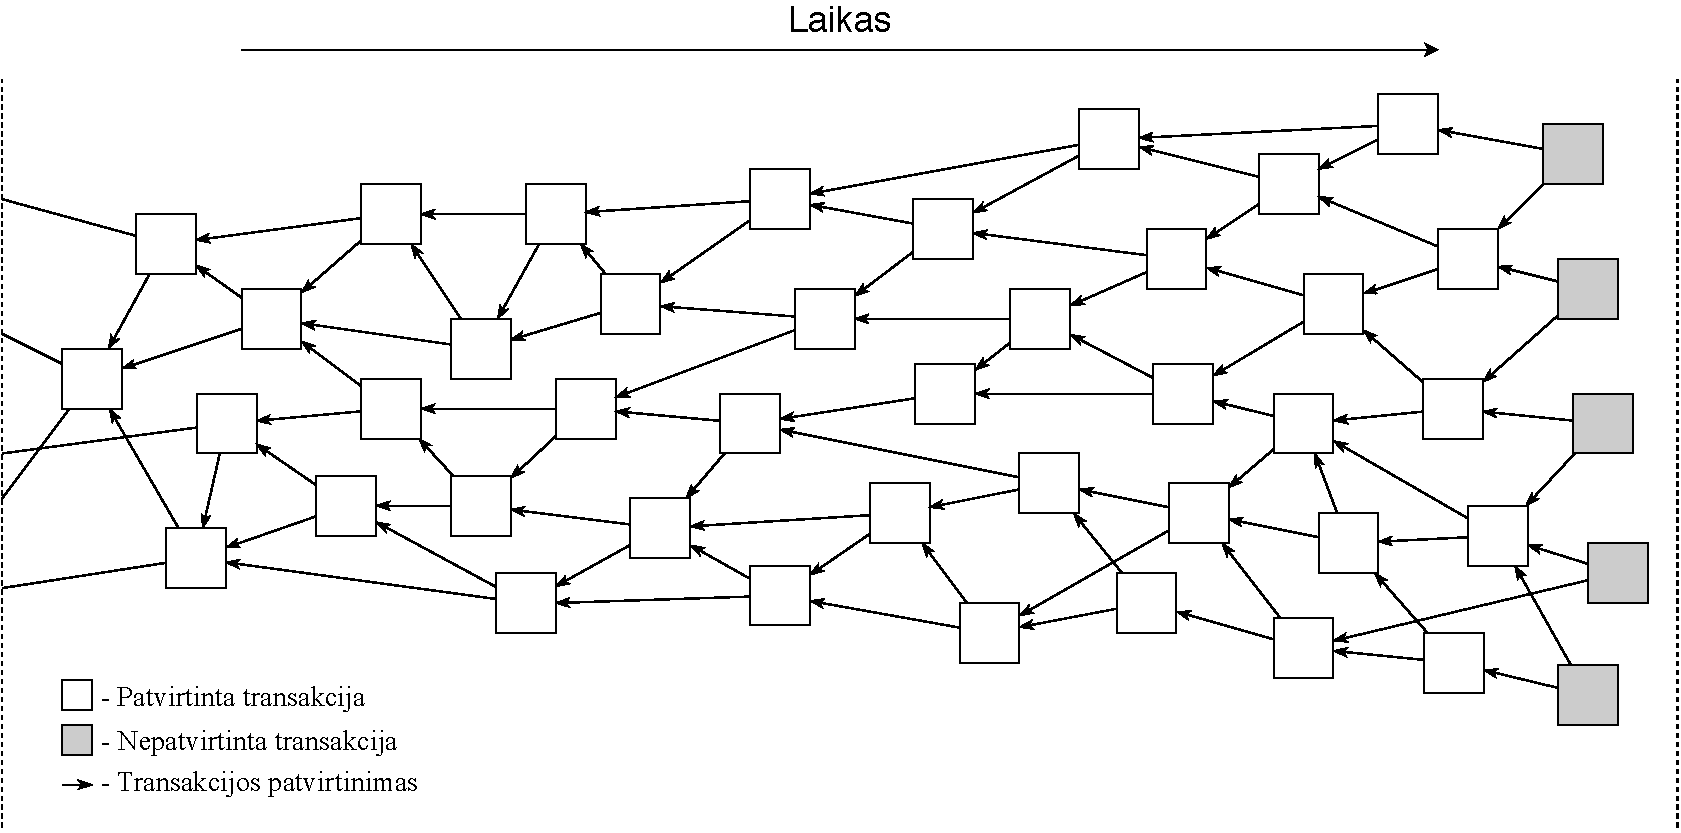
\includegraphics[scale=0.56]{images/iota-tangle}
    \caption{IOTA raizginio modelis~\cite{popov2016tangle}}
    \label{img:8}
\end{figure}

Transakcijų patvirtinimo įgyvendinimas yra unikalus ir specifinis procesas, kuriame didelę reikšmę turi matematiniai skaičiavimai. Visų pirma, norint atlikti transakciją IOTA tinkle, yra privaloma atlikti nuoseklius žingsnius: pasirinkti 2 transakcijas, patikrinti jų validumą ir atlikti darbą PoW principu~\cite{popov2016tangle}. 

Unikalu yra tai, kad kiekvienas narys, norintis atlikti transakciją, PoW atlieka pats~\cite{bramas2018stability}. Priešingai negu Bitcoin ar Ethereum, kur PoW galima deleguoti kitiems tinklo nariams, už tai sumokant transakcijos mokestį. Tačiau IOTA naudojamas PoW yra gerokai paprastesnis ir nereikalaujantis daug skaičiavimo galios~\cite{popov2016tangle}. Visų pirma, PoW reikalingas tam, kad būtų apsisaugoma nuo fiktyvių transakcijų (angl. \textit{Spam})~\cite{popov2016tangle}. Skaičiavimų sudėtingumas žemas dėl to, kad IOTA pritaikyta daiktų internetui, kuriame dalyvauja labai smulkūs prietaisai, neturintys pajėgumų sudėtingiems skaičiavimams atlikti.

Tuo tarpu transakcijų parinkimo klausimas nėra toks trivialus ir nuo to priklauso visos ekosistemos stabilumas. IOTA ir neturi jokių formalių taisyklių transakcijų parinkimo patvirtinimui, t.y. galima laisva nuožiūra pasirinkti pačiam, kokias transakcijas patvirtinti~\cite{popov2016tangle}. Tačiau egzistuoja rekomendacinis algoritmas~\cite{popov2016tangle}. Šį algoritmą renkasi dauguma tinklo narių, nes sąžiningai jo laikantis padidėja tikimybė, kad likę nariai taip pat laikysis šio algoritmo. Iš to seka, kad algoritmo besilaikančių narių transakcijos bus patvirtintos kitų narių su aukštesne tikimybe.

2 transakcijos parenkamos pagal viršūnių parinkimo algoritmą (angl. \textit{Tip Selection Algorithm}), toliau – TSA, o IOTA atveju konkrečiai – Markov Chain Monte Carlo (MCMC) algoritmu, kurio veikimui įtaką daro su kiekviena transakcija susieta informacija ir atributai~\cite{bramas2018stability}. Tai transakcijos svoris (angl. \textit{Weight}), transakcijos taškai (angl. \textit{Score}) ir transakcijos kaupiamasis svoris (angl. \textit{Cumulative Weight})~\cite{popov2016tangle}. 



% --------------------------------------------------------------- %
%                       2.2.2.2. IOTA SAUGUMAS
% --------------------------------------------------------------- %

\subsubsubsection{IOTA saugumas} \label{subsection:dag-security}

IOTA platforma buvo pradėta kurti atsižvelgus į ateities perspektyvas ir kuriamas naujas technologijas. Viena iš tokių ateities perspektyvų – kvantiniai kompiuteriai (angl. \textit{Quantum Computers}), kurie gali padaryti daugumą blokų grandinių pažeidžiamomis. Šis pažeidžiamumas kyla iš to, kaip yra atliekami PoW skaičiavimai ir kaip pasirašomos transakcijos~\cite{kiktenko2018quantum}. Pakankamai galingas kvantinis kompiuteris galėtų įvykdyti 51 procento ataką ir pakreipti visą tinklą savo naudai~\cite{kiktenko2018quantum}. 

Tai reiškia, kad Bitcoin, o kartu ir PoW konsensuso algoritmu paremtos blokų grandinės taptų nesaugios. Tačiau net jeigu blokų grandinė ir nėra paremta PoW konsensuso algoritmu, ji gali tapti nesaugi kitomis prasmėmis. Tam tikrais atvejais yra būtina paviešinti viešą raktą ir kvantinis kompiuteris, pasinaudojęs šiuo raktu, galėtų nustatyti privataus rakto reikšmę~\cite{aggarwal2017quantum}. Privatus raktas yra naudojamas pasirašant transakcijas, patvirtinant savo tapatybę bei laikant kriptovaliutas (angl. \textit{Cryptocurency}) kriptopiniginėse (angl. \textit{Crypto Wallets}). Tokia spraga reikštų, kad asmenys, disponuojantys kvantiniu kompiuteriu, galėtų perskaityti privačiu raktu užšifruotas žinutes, pasisavinti sąskaitoje laikomą turtą ar apsimesti kitu asmeniu.

IOTA savo ruožtu nepateikia visiško atsparumo kvantinių kompiuterių atakoms, tačiau teigia, kad jų sprendimas yra žymiai saugesnis, negu Bitcoin ar kitų panašių platformų. IOTA naudoja Winternitz vienkartinę parašo panaudojimo schemą, kuri, kaip manoma, yra atspari kvantiniams kompiuteriams~\cite{el2018review}.



% --------------------------------------------------------------- %
%                     2.2.2.3. IOTA PRALAIDUMAS
% --------------------------------------------------------------- %

\subsubsubsection{IOTA pralaidumas} \label{subsection:dag-throughput}

IOTA, priešingai negu blokų grandinės, neturi tokio architektūrinio vieneto kaip blokas, todėl pralaidumas ir greitis priklauso tik nuo individualių transakcijų patekimo į raizginį greičio. Žinant IOTA veikimo principą, galima išskirti rodiklius, darančius įtaką tinklo pralaidumui:
\begin{itemize}
    \item PoW skaičiavimo, kurį atlieka transakciją kuriantis narys, atlikimo laikas;
    \item Kokia tikimybė, kad transakciją patvirtins kiti nariai;
    \item Kiek ilgai kitiems tinklo nariams užtrunka patikrinti transakcijos validumą ir ją patvirtinti;
    \item Kiek tinkle yra aktyvių narių, kuriančių transakcijas.
\end{itemize}

IOTA neturi konkrečių teorinių TPS limitų. Visi apribojimai kyla iš to, kaip greitai individualių transakcijų kūrėjai apskaičiuos kiekvienai transakcijai reikalingą atlikti PoW. Taip pat, kuo daugiau aktyvių narių tinkle, tuo aukštesnis bendras TPS dydis, nes daugiau narių kuria naujas transakcijas ir daugiau narių jas tvirtina. Taigi vieninteliai technologijos limitai – tai individualių mašinų tinkle kiekis bei jų skaičiavimo ir validavimo sparta.

Kitas svarbus aspektas – transakcijų mokestis. IOTA netaiko jokio transakcijų mokesčio~\cite{zivic2019distributed}. O tai tampa pranašumu tinklo naudotojams, kurio neturi dauguma blokų grandinių naudotojų. Be to, transakcijos neprivalo perduoti kriptovaliutų. Tai reiškia, kad galima atlikti tuščias transakcijas arba tiesiog dalintis informacija su kitais tinklo nariais. Ši savybė tampa naudinga daiktų internete įrenginiams atliekant mikrotransakcijas.



% --------------------------------------------------------------- %
%        2.2.2.4. PASLĖPTI NUSTATYTOS TAPATYBĖS PRANEŠIMAI
% --------------------------------------------------------------- %

\subsubsubsection{Maskuotieji nustatytos tapatybės pranešimai} \label{subsection:dag-mam}

Tiekimo grandinėse nepaprastai svarbus duomenų atsekamumas. Daugumai grandinės narių svarbu matyti prekės judėjimą, t.y. kur ir kada prekė keliavo, kaip pasikeitė prekės laikinieji savininkai, kokia buvo prekės būsena skirtingais laiko momentais ir t.t. Be to, kai kurie duomenys yra jautrūs ir reikia suvaldyti, kuri informacija kurioms šalims turi būti prieinama, o kuri – ne. Šį darbą dažnai tenka atlikti ranka, patikrinant skirtingus informacijos šaltinius.

IOTA šiai problemai spręsti yra sukūrusi maskuotus nustatytos tapatybės pranešimus (angl. \textit{Masked Authenticated Message}), toliau – MAM. Tai yra biblioteka, užšifruojanti, iššifruojanti ir nustatanti tapatybę duomenų, kuriuos yra norima publikuoti į IOTA raizginį~\cite{andreas2017masked}. Publikuojant tokius užšifruotus duomenis, galima atskleisti specialų raktą prenumeratoriams (angl. \textit{Subscribers}), kurie turėtų teisę stebėti duomenis. Duomenų pranešėjas (angl. \textit{Publisher}) tam sukuria kanalą (angl. \textit{Channel})~\cite{ab2018iota}.

Kuriant kanalą atsiveria nemažai konfigūracijos pasirinkimų. Kanalą galima padaryti išsišakojusį, kiekvieną šaką padaryti prieinamą skirtingoms šalims ir kiekvienoje jų publikuoti skirtingą informaciją~\cite{ab2018iota}. Taip pat galima nustatyti norimą kanalo privatumo režimą iš 3 galimų rūšių~\cite{paul2017introducing}:
\begin{itemize}
    \item Viešas (angl. \textit{Public}), kuriame skelbiama informacija yra prieinama absoliučiai kiekvienam IOTA tinklo nariui.
    \item Privatus (angl. \textit{Private}), kurį gali iššifruoti šalis, turinti specialų raktą. Naudinga įrenginių tarpusavio komunikacijai.
    \item Suvaržytas (angl. \textit{Restricted}), kurį gali iššifruoti šalis, turinti specialų raktą, bei turinti autorizacijos raktą. Šis režimas leidžia kanalo iniciatoriui nutraukti transliavimą šalims, turinčioms tam tikrą autorizacijos raktą nepakeičiant specialaus rakto reikšmės. Nustačius naują autorizacijos raktą galima nustatyti, kam bus suteiktos naujos prenumeratorių teisės.
\end{itemize}

Supaprastintas MAM veikimo modelis pavaizduotas ~\ref{img:9} pav. Duomenų pranešėjas siunčia žinutes, kurias stebi 3 prenumeratoriai. Pirmajam pranešėjas atskleidė specialų ir autorizacijos raktą, todėl jis gali iššifruoti ir perskaityti visų kanalų žinutes. Antrasis prenumeratorius turi specialų raktą, todėl gali skaityti privataus ir viešo kanalo žinutes, tačiau negali iššifruoti suvaržyto kanalo žinučių. Trečiasis prenumeratorius gali skaityti tik viešojo kanalo žinutes, t.y. trečią ir šeštą žinutes.

\begin{figure}[H]
    \centering
    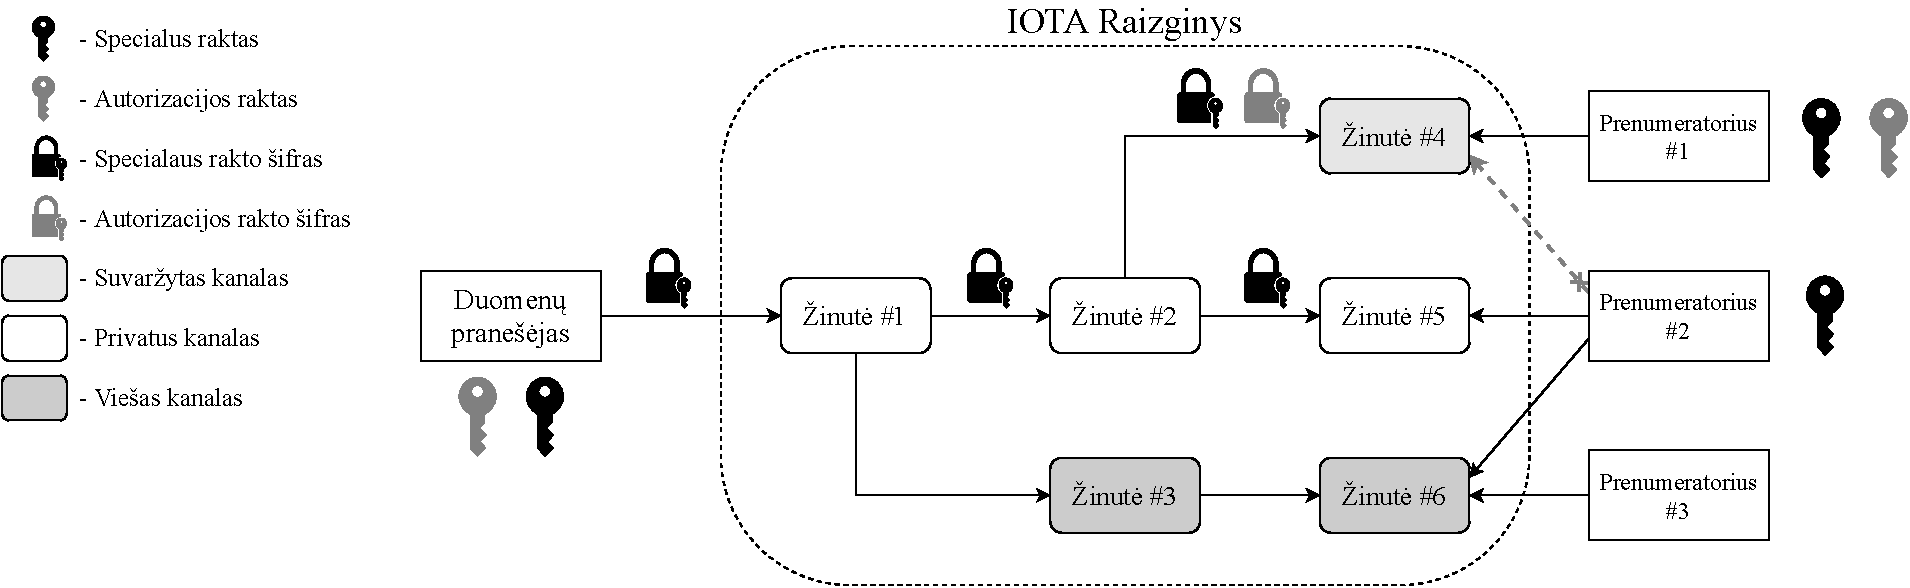
\includegraphics[scale=0.51]{images/mam-example}
    \caption{MAM supaprastintas modelis}
    \label{img:9}
\end{figure}



% --------------------------------------------------------------- %
%               2.2.2.5. KVORUMU PAREMTI SKAIČIAVIMAI
% --------------------------------------------------------------- %

\subsubsubsection{Kvorumu paremti skaičiavimai} \label{subsection:dag-qubic}

Kaip jau nagrinėta~\ref{subsection:blockchain-drawbacks} poskyryje, išmanieji kontraktai praturtina blokų grandines. Ne išimtis ir IOTA. To pagrindu IOTA platformoje kaip atskiras sluoksnis yra kuriamas kvorumu paremtų skaičiavimų protokolas (angl. \textit{Quorum Based Computations}), toliau – Qubic, sudarytas iš 3 esminių dedamųjų.

Pirmoji – orakulai (angl. \textit{Oracles}), atliekantys tinklo tarpininko su išoriniu pasauliu vaidmenį~\cite{iota2017oracles}. Galimas to pavyzdys – IOTA tinklas negali žinoti tiekimo grandinėse galimų rizikų, sukeltų gamtos stichijų ar kitų grandinės narių, kurių nemaža dalis aprašyta šaltiniuose~\cite{behdani2012handle, strom2013pwc}, poveikio ir dydžio. Orakulas šią informaciją galėtų surinkti ir transliuoti ją tinklui. Tačiau šia informacija orakulai gali manipuliuoti savo naudai. Kad to būtų išvengta, išorinio pasaulio faktų validumas turi būti priimtas kvalifikuota dauguma – kvorumu, t.y. ne mažiau nei 2/3 visų orakulų turi pateikti sutampančią informaciją~\cite{iota2017oracles}. Taip pat egzistuoja ir kiti apsaugos mechanizmai, tokie kaip paskatos už teisingų rezultatų transliavimą, sankcijos už bandymus manipuliuoti informacija ir pan.

Antroji Qubic dedamoji – paskirstyti skaičiavimai~\cite{iota2017oracles}. Daiktų internete smulkiems įrenginiams gali tekti susidurti su sudėtingais skaičiavimais, kurių šie įrenginiai nepajėgtų išspręsti arba tai užtruktų per daug laiko. Qubic protokolas įgalintų perduoti (angl. \textit{Outsource}) šiuos skaičiavimus išorinėms ir gerokai galingesnėms mašinoms, kurios grąžintų skaičiavimų rezultatus smulkiems įrenginiams.

Paskutinė Qubic protokolo dalis – išmanieji kontraktai. Išmanieji kontraktai pasižymi savybe: žinodami, kokius įvesties duomenis paduosime kontraktui, taip pat žinosime, kokio rezultato iš jo tikėtis~\cite{iota2017oracles}. Ši savybė leidžia juos pritaikyti realizuojant mašinų tarpusavio bendravimą (angl. Machine to Machine), toliau – M2M. Taip pat būtų galima automatizuoti informacijos apsikeitimą, bendravimą su prieš tai minėtais orakulais, bei paskirstytų skaičiavimų inicijavimą.

Qubic įgyvendinimas iš dalies yra panašus į turimos įtakos konsensuso algoritmą (angl. \textit{Proof of Stake}), toliau – PoS, kurį turi įgyvendinę dalis blokų grandinių bei prie kurio ateityje ketina pereiti Ethereum platforma\footnote{Informacija iš: \href{https://docs.ethhub.io/ethereum-roadmap/ethereum-2.0/proof-of-stake}{https://docs.ethhub.io/ethereum-roadmap/ethereum-2.0/proof-of-stake} [žiūrėta 2019-05-17].}. PoS efektyvina tinklo naudojamus resursus, likviduodama PoW atliekamą darbą mašinoms bei pašalindama globalaus konsensuso poreikį smulkiems dalykams. Taigi, vietoje to, kad validavimą, skaičiavimus bei balsavimą dėl visų išorinio pasaulio faktų atliktų kiekvienas tinkle esantis narys, šį darbą padaro orakulai.



% --------------------------------------------------------------- %
%               2.2.2.6. EKONOMINIS KLASTERIZAVIMAS
% --------------------------------------------------------------- %

\subsubsubsection{Ekonominis klasterizavimas} \label{subsection:dag-ec}

Ekonominis klasterizavimas (angl. \textit{Economic Clustering}), toliau EC – samprata, pristatyta Sergey Ivancheglo ir įgalinanti IOTA platformos plečiamumą, kitaip – neribotą TPS kiekį~\cite{sergey2018economic}.
Ekonominis klasteris – tai grupė prietaisų, esančių konkrečiame regione: kontinente, valstybėje, kelio ruože ar pastate~\cite{sergey2018economic}. 

Pati idėja yra glaudžiai susijusi su daiktų internetu, o klasterių struktūra priklauso nuo ekonominės veiklos tame regione~\cite{sergey2018economic}. IOTA platforma naudojasi vartotojai iš bet kurios pasaulio vietos, bet tai nėra efektyvu. Pavyzdžiui, JAV įsikūrusio fabriko temperatūros jutikliui nėra aktualu Kinijos piliečio transakcija savo draugui, gyvenančiam už kelių kvartalų. Tačiau jutiklis, norėdamas atlikdamas informacinę transakciją klientui, tikėtina, kad turės validuoti ir patvirtinti būtent jam neaktualią transakciją iš Kinijos. O juk būtų logiškiau, jeigu fabriko prietaisai turėtų prieigą tik prie jiems aktualių transakcijų ekonominiame regione.

EC išsidėstymo modelis pavaizduotas~\ref{img:10} pav. Kiekviename klasteryje yra lokaliai vykdomos IOTA transakcijos. Pavyzdžiui, 0 klasteris gali atlikti transakcijas 0 klasteryje, 1 klasteriui ir 2 klasteriui. Tačiau 0 ir 3 klasteris nėra kaimynai ir vienas kito transakcijų nemato, todėl jas ignoruoja. Jeigu iškiltų poreikis 0 klasterio nariui atlikti transakciją 3 klasteryje, šiam nariui tektų atlikti transakciją sau pačiam į 1 arba 2 klasterį, tada iš jo atlikti transakciją sau į 3 klasterį ir atlikti transakciją 3 klasteryje.

\begin{figure}[H]
    \centering
    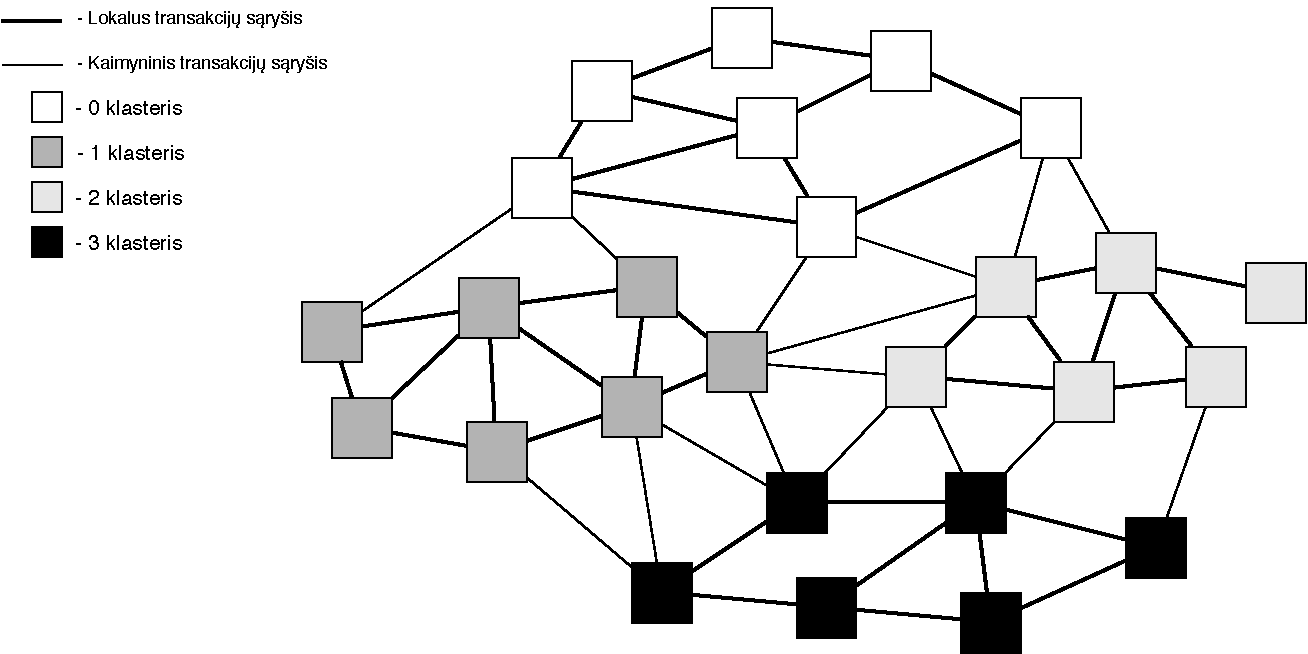
\includegraphics[scale=0.7]{images/economic-clusters}
    \caption{Ekonominio klasterizavimo modelis}
    \label{img:10}
\end{figure}

Tačiau iš EC modelio kyla tam tikri trūkumai ir rizikos~\cite{sergey2018economic}: 
\begin{itemize}
    \item Sunkumai atliekant transakcijas į tolimus klasterius;
    \item Dažnai tenka pervedinėti valiutą sau pačiam;
    \item Klasteriai gali kurti savo valiutą, kurios vertė kituose klasteriuose gali skirtis.
\end{itemize} 



% --------------------------------------------------------------- %
%            2.2.2.7. DALYVAVIMAS TINKLE NEPRISIJUNGUS
% --------------------------------------------------------------- %

\subsubsubsection{Dalyvavimas tinkle neprisijungus} \label{subsection:dag-offline}

Transportuojant krovinius gali tekti atsidurti situacijose, kai interneto ryšys yra nepasiekimas. Svarbu, kad darbas tęstųsi net ir trumpam dingus internetui. Pavyzdys – krovinių plukdymas per vandenyną. Naudojama technologija turi užtikrinti stabilų veikimą be interneto, ir kad atsiradus interneto ryšiui nebūtų pateikiami suklastoti duomenys.

Šiuo klausimu IOTA yra pranašesnė už Bitcoin ir Ethereum, nes įgalina transakcijas neturint interneto ryšio~\cite{zivic2019distributed}. Transakcijų vykdymas periode be interneto pavaizduotas~\ref{img:11} pav. Naudotojas X, dingus internetui, mato visas transakcijas, išskyrus tas, kurias likęs tinklas atlieka naudotojui X neturint interneto ryšio. Vienintelė logiška veiksmų seka naudotojui X yra susikurti savo atskirą raizginį (angl. \textit{sub-tangle}), kuriame X transakcijos tvirtins X transakcijas.

\begin{figure}[H]
    \centering
    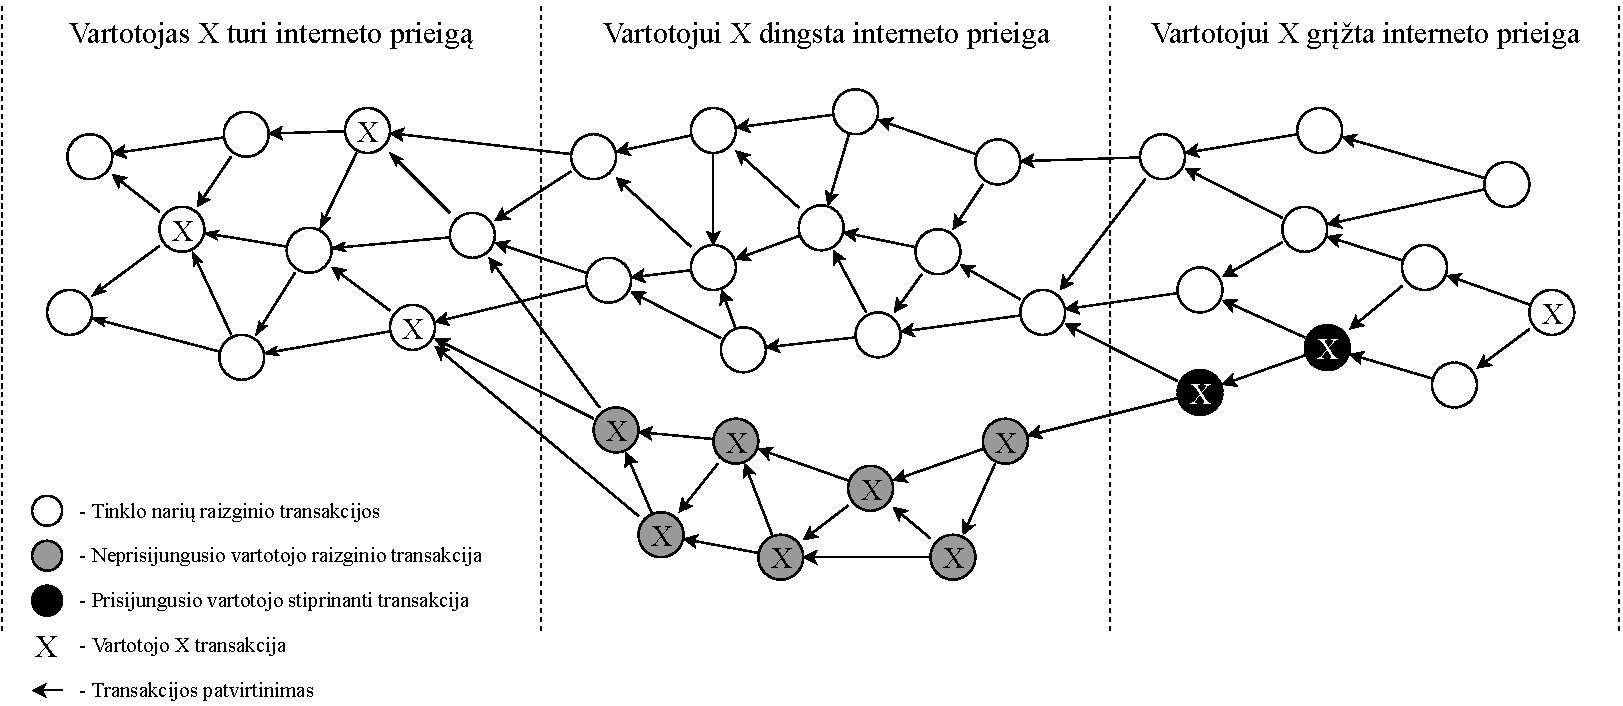
\includegraphics[scale=0.6]{images/offline-tangle}
    \caption{Transakcijų vykdymas neturint interneto prieigos}
    \label{img:11}
\end{figure}

Atsiradus interneto prieigai dar nereiškia, kad vartotojo X atskiras raizginys bus patvirtintas, todėl reikia atlikti specialias stiprinančias transakcijas, kurios padidina šansus, kad tinklas palaipsniui pripažins ir validuos atskirą raizginį kaip tinkamą įtraukti į bendrą tinklą~\cite{bennet2017technical}. Stiprinanti transakcija būtinai turi patvirtinti vieną pagrindinio raizginio ir vieną atskiro raizginio X transakciją~\cite{bennet2017technical}. Kuo daugiau stiprinančių transakcijų, tuo didesnė validavimo tikimybė, tačiau yra reikalingos bent 2 stiprinančios transakcijos~\cite{bennet2017technical}.



% --------------------------------------------------------------- %
%  2.3. BLOKŲ GRANDINĖS IR ORIENTUOTO GRAFO BE CIKLŲ PALYGINIMAS
% --------------------------------------------------------------- %

\subsection{Blokų grandinės ir orientuoto grafo be ciklų palyginimas} \label{subsection:dlt-compare}

Taigi, galima apibendrinti pagrindinius skirtumus tarp DAG ir blokų grandinių principais paremtų DLT. Architektūra yra akivaizdžiausias skirtumas. Blokų grandinė yra tiesinės formos darinys, sudarytas iš nuosekliai sujungtų blokų, o DAG yra raizginys, sudarytas iš individualių transakcijų. Tačiau iš to kyla IOTA trūkumas – palankesnės sąlygos piktybinių transakcijų kūrimui. Blokų grandinėse sukurti atskirą piktybinių blokų atšaką yra gerokai sudėtingiau ir reikalauja daugiau resursų negu kuriant atskirą transakcijų grandį IOTA tinkle. Tačiau nuogąstauti dėl tinklo pažeidžiamumo nėra pagrindo. Tam, kad būtų pažeistas duomenų nekintamumas, abiem atvejais kenkėjo skaičiavimo resursai turi būti didesni nei viso likusio tinklo.

Abi DLT atmainos naudoja PoW skaičiavimus, tačiau IOTA tinkle kiekvienas narys juos atlieka individualiai. Tuo tarpu blokų grandinėse šį procesą galime deleguoti. Esant aukštam PoW skaičiavimų sudėtingumui, tai tampa trūkumu tiekimo grandinėse. Jeigu daiktų internetas taptų visuotinai naudojama technologija logistikoje, transakcijas arba apsikeitimą duomenimis turėtų atlikti net ir patys smulkiausi prietaisai, nepasižymintys didele skaičiavimo galia.

Dar vienas IOTA trūkumas yra koordinatorius. Šiuo metu pastaroji pltforma yra ankstyvoje fazėje ir negali savarankiškai funkcionuoti, todėl ją turi prižiūrėti specialus agentas, vadinamas koordinatoriumi~\cite{bramas2018stability}. Yra teigiama, kad tai pažeidžia vieną iš pagrindinių DLT principų – nepriklausomumą nuo trečiųjų šalių. Šiuo atžvilgiu blokų grandinės lenkia IOTA, nes gali veikti autonomiškai, be trečiosios šalies įsikišimo. Vis dėlto IOTA kūrėjai ateityje tikisi pašalinti koordinatoriaus poreikį~\cite{bramas2018stability}.

Saugumo klausimu IOTA turi pranašumą kvantinių kompiuterių atžvilgiu, tačiau tai yra labiau aktualu ilgojoje perspektyvoje. Kol kas nėra sukurtų galingų, pigių ir plačiai naudojamų kvantinių kompiuterių, todėl šis privalumas šiandien nėra lemiamas veiksnys renkantis tarp šių dviejų DLT tipų. Be to, blokų grandinės laikui bėgant galėtų prisitaikyti prie kvantinių kompiuterių keliamų grėsmių pakeisdamos savo architektūrinius sprendimus.

Ko gero didžiausią įtaką technologijos pasirinkimui lemia rodikliai, susiję su atliekamų transakcijų greičiu ir kaina. Tiekimo grandinėms yra svarbu, kad transakcijos apsimokėtų, t.y. įvyktų kuo greičiau ir pigiau. Svarbu lyginti rodiklius, darančius įtaką maksimaliai tinklo apkrovai, vienos transakcijos įvykdymo laikui ir finansinei naudai. Didžioji dalis blokų grandinių turi TPS limitus arba transakcijos mokestį, o IOTA – ne. Taigi, pritaikius IOTA tiekimo grandinėse, būtų galima dalintis informacija už dyką ir labai greitai, sutaupant daug resursų visuose grandies procesuose.

IOTA taip pat įgalina transakcijas neprisijungus ir MAM, sukuriančius potencialių technologijos panaudojimo atvejų, o pilnai įgyvendinus kvorumu paremtus skaičiavimus ir ekonominį klasterizavimą, jų atsirastų dar daugiau.

Nepaisant visų IOTA trūkumų, remiantis jos savybių ir rodiklių pranašumais blokų grandinių atžvilgiu bei sąlygomis daiktų internetui, galima teigti, jog būtent ši DLT atmaina yra palankesnė taikymui tiekimo grandinių ir logistikos srityje. Taigi, toliau pasirinkta konstruoti panaudojimo scenarijus tiekimo grandinės procesuose naudojant IOTA platformą.
% --------------------------------------------------------------- %
%             3. IOTA PANAUDOJAMUMAS TIEKIMO GRANDINĖSE 
% --------------------------------------------------------------- %

\section{IOTA platformos panaudojimas tiekimo grandinėse} \label{section:application}



% --------------------------------------------------------------- %
%                   3.1. TIEKIMO GRANDINĖS ATVEJIS
% --------------------------------------------------------------- %

\subsection{Tiekimo grandinės atvejis} \label{subsection:sc-example}

Tiekimo grandinės pavyzdinis atvejis buvo kuriamas šio darbo autoriaus, remiantis kelių šaltinių pavyzdinėmis idėjomis~\cite{christopher2016logistics, webber2009building, patrick2017continuous, justin2016customer}. Naudojantis jomis buvo sukurta viena bendra diagrama (žr. priedą~\ref{appendix:1}). 

Diagrama nebuvo siekiama pavaizduoti realaus pasaulio tiekimo grandinės pavyzdžio\footnote{Dėl konfidencialumo priežasčių įmonės nėra linkusios skelbti oficialių savo tiekimo grandinių modelių.}, o labiau siekta sukurti modelį, apimantį kuo daugiau skirtingų tiekimo grandinės fazių ir etapų, kad tai leistų geriau atskleisti IOTA platformos panaudojamumą. Pateiktas modelis galėjo būti dar detalesnis, tačiau tai nebūtinai atspindėtų norimos perteikti esmės.

Šis teikimo grandinės atvejis vaizduoja supaprastintą vaisių tiekimo grandinę nuo ūkininko, įsigyjančio sėklas iki kliento, perkančio vaisius prekybos centre. Tiekimo grandinė išskaidyta į 15 diskrečių etapų, kurių kiekvienas aprašytas atitinkamai.

\medskip \noindent \textbf{1. Ūkininkas superka sėklas iš tiekėjo.} Prieš tai yra sudaromas raštiškas kontraktas tarp sėklų tiekėjo ir ūkininko, kad už tam tikrą kainą ūkininkas gaus tam tikrą kiekį sėklų. Be to, sutartyje gali būti papildomų sąlygų, jei sėklų tiekėjas laiku neturės sėklų arba jų kokybė neatitiks keliamų standartų.

\medskip \noindent \textbf{2. Ūkininkas nurenka pasėtą derlių.} Ūkininkas pasėja vaisių sėklas, sudaro tinkamas sąlygas jų auginimui ir atėjus laikui užaugintus vaisius nurenka ir sandėliuoja. 

\medskip \noindent \textbf{3. Ūkininkas parduoda derlių supirkėjui.} Pardavimas vyksta pagal iš anksto sudarytą kontraktą. Ūkininkas įsipareigoja atėjus konkrečiam terminui parduoti supirkėjui atitinkamą kiekį vaisių, tenkinančių nustatytą kokybės standartą už atitinkamą kainą.

\medskip \noindent \textbf{4. Kurjeris pakrauna vaisius į sunkvežimį.} Supirkėjas samdo kurjerį iš logistikos įmonės, teikiančios transportavimo paslaugas. Supirkėjas gali šiam darbui paskirti ir savo darbuotojus, atsakingus už prekių transportavimą. Pirmuoju atveju būtų sudaromas kontraktas tarp supirkėjo ir logistikos įmonės, įsipareigojančios atgabenti nepažeistas prekes iki nustatyto termino.

\medskip \noindent \textbf{5. Vaisiai transportuojami iki fabriko.}

\medskip \noindent \textbf{6. Vaisiai apdirbami (pagaminami jų išvestiniai produktai) ir sandėliuojami.} Priklausomai nuo vaisių supirkėjo veiklos srities, jis gali vaisius paruošti pardavimui, pvz. apipurkšti cheminiu produktu, suteikiantį blizgumą ar atsparumą, taip pat apdirbti juos supjaustant, panaudojant kaip sudedamąją dalį kituose produktuose ir t.t. Galutiniai produktai sandėliuojami fabriko patalpose, kol atvyks kurjeriai, atsakingi už prekių transportavimą į prekybos centrus. Su prekybos centrais yra pasirašomi kontraktai, nustatantys, kokius produktus už kokią kainą vaisių supirkėjas parduos prekybos centrui.

\medskip \noindent \textbf{7. Apdirbti vaisiai pakraunami į sunkvežimį.} Čia kurjeris gali būti samdomas tuo pačiu principu, kaip ir 4 etape.

\medskip \noindent \textbf{8. Vaisiai transportuojami į jūrų uostą.} Jūrų uostas pagal vidines taisykles perima konteinerį ir paruošia jį pakrovimui į laivą.

\medskip \noindent \textbf{9. Vaisių konteineriai pakraunami į krovininį laivą.}

\medskip \noindent \textbf{10. Krovininis laivas nuplaukia į kitą uostą.}

\medskip \noindent \textbf{11. Vaisių konteineriai iškraunami į sunkvežimius.} Tikėtina, kad kurjeris yra iš tos pačios logistikos kompanijos, kurios sunkvežimis nuvežė konteinerį į pirmąjį jūrų uostą.

\medskip \noindent \textbf{12. Sunkvežimiai išvežioja vaisius į skirtingas šalis.} Transportuojant vaisius yra pasiekiama kitos valstybės siena, kur kurjeris susiduria su muitine.

\medskip \noindent \textbf{13. Muitinėse patikrinami kroviniai.} Priklausomai nuo valstybės, už krovinio įvežimą į šalį gali būti taikomi skirtingi mokesčiai, o kroviniui taikomos skirtingos taisyklės ir standartai. Už atsiskaitymą su muitine yra atsakingas prekybos centras, norintis įsivežti prekes. Atlikus visas būtinas procedūras muitinė išduoda specialų leidimą.

\medskip \noindent \textbf{14. Vaisiai išvežiojami į prekybos centrus.}

\medskip \noindent \textbf{15. Vaisiai parduodami galutiniams pirkėjams.}



% --------------------------------------------------------------- %
%    3.2. TIEKIMO GRANDINĖS ATVEJIS PRITAIKIUS IOTA PLATFORMĄ
% --------------------------------------------------------------- %

\subsection{Tiekimo grandinės atvejis pritaikius IOTA platformą} \label{subsection:application-iota}

Šiame skyriuje autorius pateikia pavyzdinius tiekimo grandinės modelius pritaikius IOTA platformos savybes. Kiekvienas papildytas panaudojimo atvejo etapas arba etapai aprašyti atskirai poskyriuose, pateikiant diagramą su kiekvienu etapo žingsnio detaliu aprašymu.



% --------------------------------------------------------------- %
%                       3.2.1 PIRMAS ETAPAS
% --------------------------------------------------------------- %

\subsubsection{Pirmas etapas} \label{subsection:uc-1}

Pirmojo etapo papildytas modelis, \textit{Ūkininkas superka sėklas iš tiekėjo} (žr.~\ref{img:12} pav.):
\begin{enumerate}
    \item Tarp sėklų pardavėjo ir ūkininko yra sudaromas kontraktas, kad už tam tikrą sumą tam tikru metu ūkininkas galės įsigyti tam tikrą kiekį sėklų. Kontraktas pasirašomas ūkininko ir sėklų tiekėjo, o elektroninė sandorio versija užšifruojama raktu ir gautas šifras patalpinamas į IOTA raizginį. Abi šalys gauna dokumento kopiją ir šifro raktą. Niekas iš IOTA tinklo narių, išskyrus abi kontrakto šalis, negali peržiūrėti kontrakto turinio. Kontrakto šalys gali įrodyti turimos kontrakto kopijos autentiškumą užšifruodami šią kopiją ir patikrindami gauto šifro reikšmę su raizginyje esančiu šifru. Tai leidžia apsisaugoti nuo dokumentų padirbimo arba praradimo juos pametus. 
    \item Sėklų tiekėjas IOTA raizginyje sukuria MAM kanalą, kurį užsiprenumeruoja ūkininkas. Kanalas yra privatus, todėl sėklų tiekėjas prieš tai perduoda specialų raktą ūkininkui, kuris leidžia apsisaugoti, kad duomenų nematytų pašaliniai asmenys. Kanalu perduodami duomenys rašomi į raizginį, o ūkininkas realiu laiku gali stebėti sėklų būseną, pavyzdžiui lokaciją, sandėliavimo sąlygas ir pan.
    \item Sėklų tiekėjas pristato sėklas ūkininkui, o ūkininkas atlieką finansinį pavedimą tiekėjui.
\end{enumerate}

\begin{figure}[H]
    \centering
    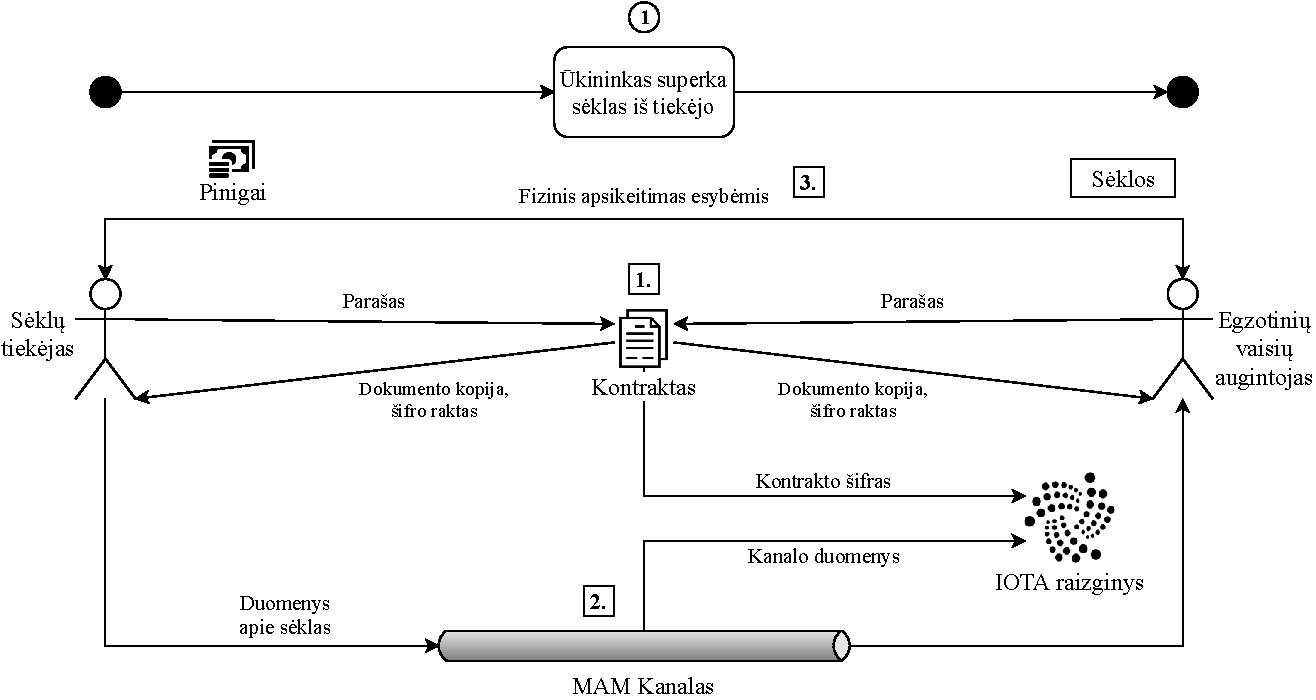
\includegraphics[scale=0.74]{images/iota-usecase-1}
    \caption{1 etapo papildytas modelis}
    \label{img:12}
\end{figure}



% --------------------------------------------------------------- %
%                       3.2.2 ANTRAS ETAPAS
% --------------------------------------------------------------- %

\subsubsection{Antras etapas} \label{subsection:uc-2}

Antrojo etapo papildytas modelis, \textit{Ūkininkas nurenka pasėtą derlių} (žr.~\ref{img:13} pav.):
\begin{enumerate}
    \item Iš pradžių ūkininkas inicijuoja privatų MAM kanalą, kuriuo siųs duomenis potencialiems derliaus supirkėjams. Ūkininkas perduoda kanalo prenumeratos raktą supirkėjui.
    \item Ten, kur yra pasodintos sėklos, pastatomi jutikliai, renkantys duomenis apie aplinką. Šie jutikliai siunčia kanalu duomenis apie vaisių auginimo sąlygas: drėgmę, temperatūrą ir kt. Jutiklius galima būtų sukonfigūruoti, kad kiekvienas atskirai siųstų duomenis į MAM kanalą, arba perduotų duomenis į ūkininko kompiuterį, kuris perimtų duomenų publikavimą.
    \item Esant poreikiui, specialūs IOTA orakulų rolę prisiėmę inspektoriai gali atlikti patikrą, ar jutiklių siunčiami duomenys nėra klastojami ir savo matavimus taip pat patalpinti IOTA raizginyje. Specialūs orakulai galėtų prisidėti ir prie kitų reikalavimų laikymosi patikros. Pavyzdžiui, ar ūkininkas auginimo metu neteršia aplinkos, ar nėra darbinami vaikai ir t.t. Orakulai gali prisidėti ir prie draudimo įmonių veiklos. Esant sausrai ir ūkininkui nepristačius pakankamai derliaus, draudimo kompanijos, gavusios patvirtinimą iš orakulų apie stichinę nelaimę, galėtų padengti ūkininkų nuostolius. Orakulų turėtų dalyvauti kuo daugiau, šitaip užtikrinant, kad daugumos jų parodymai yra objektyvūs ir sutampa. Be orakulų būtų sunku nustatyti, ar jutiklių duomenys, kuriuos teikia ūkininkas, yra nepadirbti. Orakulas duomenis gali perduoti naudojant MAM kanalą.
\end{enumerate}

\begin{figure}[H]
    \centering
    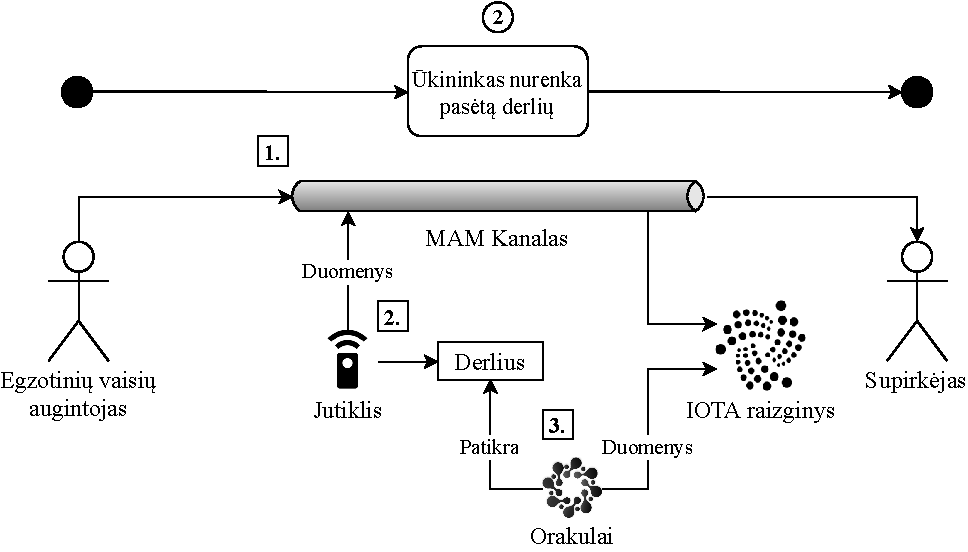
\includegraphics[scale=0.82]{images/iota-usecase-2}
    \caption{2 etapo papildytas modelis}
    \label{img:13}
\end{figure}



% --------------------------------------------------------------- %
%                       3.2.3 TREČIAS ETAPAS
% --------------------------------------------------------------- %

\subsubsection{Trečias etapas} \label{subsection:uc-3}

Trečiojo etapo, \textit{Ūkininkas parduoda derlių supirkėjui} modelio papildymas yra beveik identiškas pirmojo etapo modelio papildymui. Šiuo atveju kontraktas tarp ūkininko ir supirkėjo gali būti sudaromas prieš antrą, o esant poreikiui, ir prieš pirmą etapą tam, kad būtų galima lengviau sekti įsipareigojimų vykdymą.

Svarbu pabrėžti, kad sutarčių ir kontraktų gali būti daugiau nei vienas. Į IOTA tinklą tiekimo grandinės nariai gali įkelti neribotą kiekį bet kokio tipo reikalingų dokumentų.



% --------------------------------------------------------------- %
%                3.2.4 KETVIRTAS IR PENKTAS ETAPAI
% --------------------------------------------------------------- %

\subsubsection{Ketvirtas ir penktas etapai} \label{subsection:uc-4-5}

Ketvirtojo ir penktojo etapų, \textit{Kurjeris pakrauna vaisius į sunkvežimį} ir \textit{Vaisiai transportuojami iki fabriko} bendras papildytas modelis (žr.~\ref{img:14} pav.):
\begin{enumerate}
    \item Pakrovęs vaisius į sunkvežimį kurjeris sukuria MAM kanalą šitaip patvirtinantis perėmęs krovinį ir perimantis atsakomybę už jį\footnote{Paprastai kaskart atlikus transakciją perduodant krovinį, kartu perduodama ir atsakomybė už jį. Tai reiškia, kad krovinį perimanti šalis turi patikrinti krovinio būklę ir su kroviniu susijusius dokumentus, kad būtų galima atrasti pažeidimo priežastį ir kaltininką.}. MAM kanalą prenumeruoja fabrikas\footnote{Šiame tiekimo grandinės pavyzdinio atvejo kontekste fabrikas priklauso supirkėjui.}.
    \item Į MAM kanalą yra perduodami duomenys iš aplinkos jutiklio apie sunkvežimyje esančio krovinio sąlygas ir sunkvežimio lokaciją. Fabrikui (supirkėjui) tai yra naudinga, nes fabrikas gali reaguoti į vaisių atvežimą, pasiruošti jam. Be to, jei vaisiai vėluotų, dingtų bei būtų pristatyti pažeisti arba neatitinkantys kokybės, būtų aišku, kur incidentas įvyko ir kas už tai yra atsakingas.
    \item Vaisiai pristatomi į fabriką, kur yra perduodama atsakomybė už juos.
\end{enumerate}

\begin{figure}[H]
    \centering
    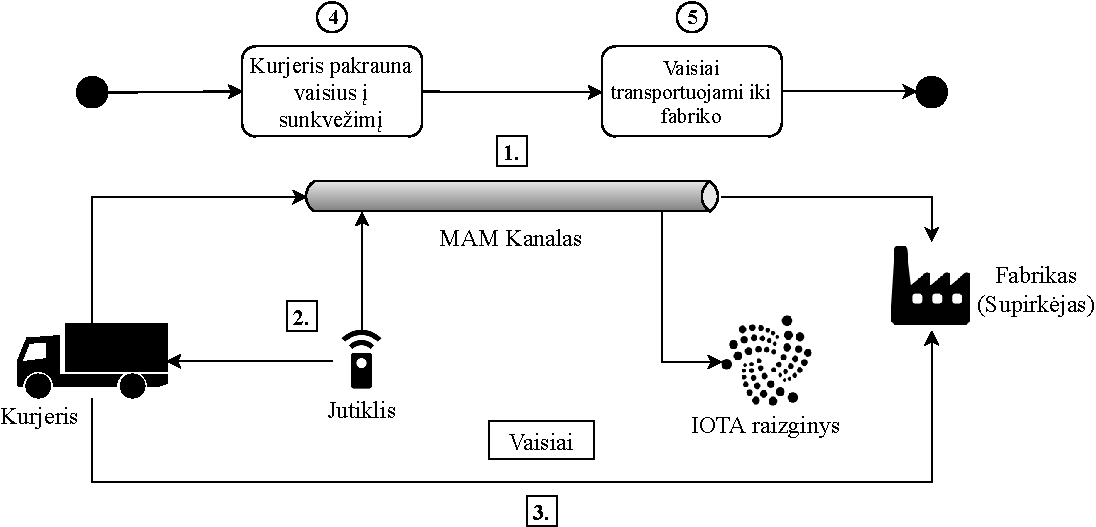
\includegraphics[scale=0.77]{images/iota-usecase-4-5}
    \caption{4 ir 5 etapų papildytas modelis}
    \label{img:14}
\end{figure}



% --------------------------------------------------------------- %
%                       3.2.5 ŠEŠTAS ETAPAS
% --------------------------------------------------------------- %

\subsubsection{Šeštas etapas} \label{subsection:uc-6}

Šeštojo etapo papildytas modelis, \textit{Vaisiai apdirbami (pagaminami jų sub-produktai) ir sandėliuojami} (žr.~\ref{img:15} pav.):
\begin{enumerate}
    \item Kaip ir pirmajame panaudojimo atvejo etape, yra sudaromas kontraktas. Fabrikas (supirkėjas) susitaria su prekybos centru, kad už tam tikrą sumą tam tikru metu bus parduotas tam tikras kiekis perdirbtų arba paruoštų vaisių. Kontraktas pasirašomas abiejų šalių, o elektroninė versija užšifruojama raktu ir gautas šifras patalpinamas į IOTA tinklą \footnote{Kontraktas gali būti sudarytas gerokai anksčiau, pavyzdžiui prieš 1 arba 2 etapą.}. Niekas iš IOTA tinklo narių, išskyrus abi kontrakto šalis, negali peržiūrėti kontrakto turinio. Kontrakto šalys gali įrodyti turimo kontrakto teisiškumą užšifruodami šią kopiją ir patikrindami gauto šifro reikšmę su raizginyje esančiu šifru.
    \item Fabrikas sukuria privatų kanalą, kurį prenumeruoja prekybos centrai\footnote{Jeigu krovinius transportuoja samdomi kurjeriai iš logistikos įmonių, kanalu duomenys gali būti siunčiami ir šiems atstovams, t.y. koks krovinių tipas, kada krovinys paruoštas transportavimui ir t.t.}. Kanalu fabrikas perduoda informaciją apie tai, kokie produktai kuriami, kurioje gamybos stadijoje šie produktai yra esamu laiko momentu, kokiais standartais vadovaujantis apdirbami ir t.t.
    \item Fabrike įtaisyti jutikliai MAM kanalu taip pat perduoda informaciją, pavyzdžiui, gamybos sąlygas skirtinguose etapuose.
    \item Esant poreikiui inspektoriai, kitaip orakulai, gali patikrinti tiek 2, tiek 3 žingsnyje fabriko teikiamą informaciją ir patalpinti į IOTA raizginį prekybos centrams pasitikrinti.
\end{enumerate}

\begin{figure}[H]
    \centering
    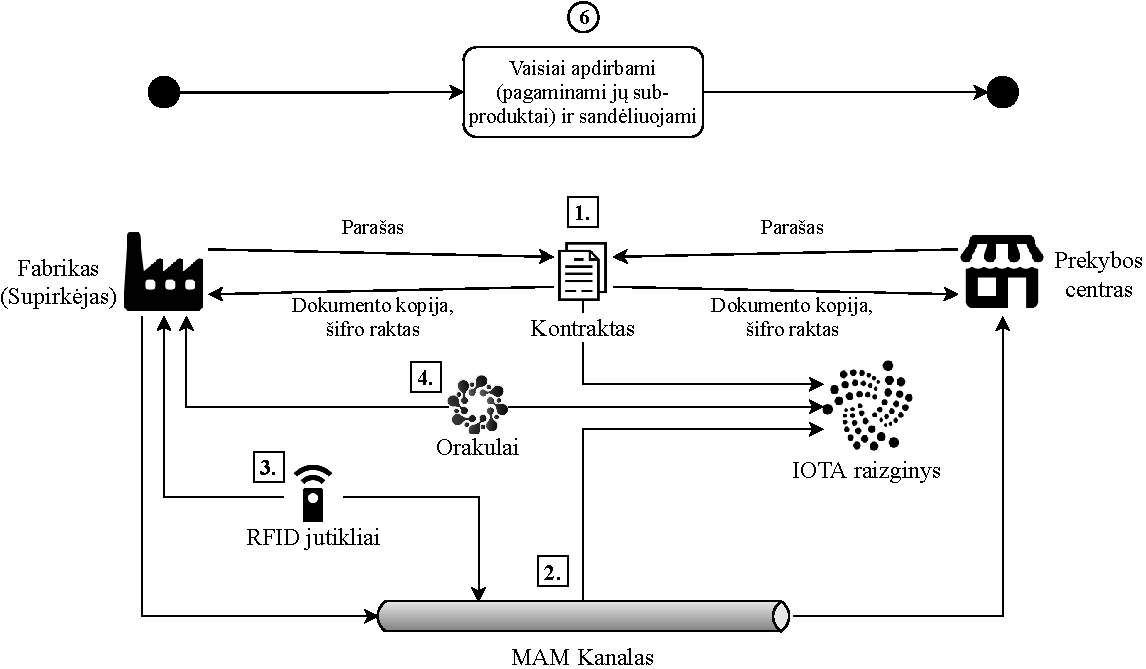
\includegraphics[scale=0.8]{images/iota-usecase-6}
    \caption{6 etapo papildytas modelis}
    \label{img:15}
\end{figure}



% --------------------------------------------------------------- %
%               3.2.6 SEPTINTAS IR AŠTUNTAS ETAPAI
% --------------------------------------------------------------- %

\subsubsection{Septintas ir aštuntas etapai} \label{subsection:uc-7-8}

Septintojo ir Aštuntojo etapų, \textit{Apdirbti vaisiai pakraunami į sunkvežimį} ir \textit{Vaisiai transportuojami į jūrų uostą} bendras papildytas modelis yra beveik identiškas atitinkamai ketvirtojo ir penktojo etapų bendram papildytam modeliui. Kurjeriui sukūrus MAM kanalą, jį prenumeruoja ne tik prekybos centras, bet ir jūrų uostas, kad būtų pasiruošta sunkvežimio atvykimui.



% --------------------------------------------------------------- %
%                3.2.7 DEVINTAS IR DEŠIMTAS ETAPAI
% --------------------------------------------------------------- %

\subsubsection{Devintas ir dešimtas etapai} \label{subsection:uc-9-10}

Devintojo ir dešimtojo etapų, \textit{Vaisių konteineriai pakraunami į krovininį laivą} ir \textit{Krovininis laivas nuplaukia į kitą uostą} bendras papildytas modelis (žr.~\ref{img:16} pav.):
\begin{enumerate}
    \item Vaisių konteineris pakraunamas į krovininį laivą.
    \item Laivas sukuria MAM kanalą, kurį užprenumeruoja kurjeris, laukiantis krovinio jūrų uoste nr. 2. Kanalu perduodama konteinerio su vaisiais laikymo sąlygos, gaunamos iš jutiklių. Laivas išplaukia iš jūrų uosto nr. 1
    \item Laivui plaukiant jūra, dingsta interneto ryšys, tačiau informacijos tiekimas nėra nutraukiamas ir informacijos transakcijos yra toliau atliekamos neprisijungus. 
    \item Po kiek laiko interneto ryšys grįžta ir visos iki tol siųstos žinutės atsiduria IOTA raizginyje, kurias prenumeruotojas gali gauti ir matyti iškart.
    \item Vaisiai transportuojami į jūrų uostą nr. 2.
\end{enumerate}

\begin{figure}[H]
    \centering
    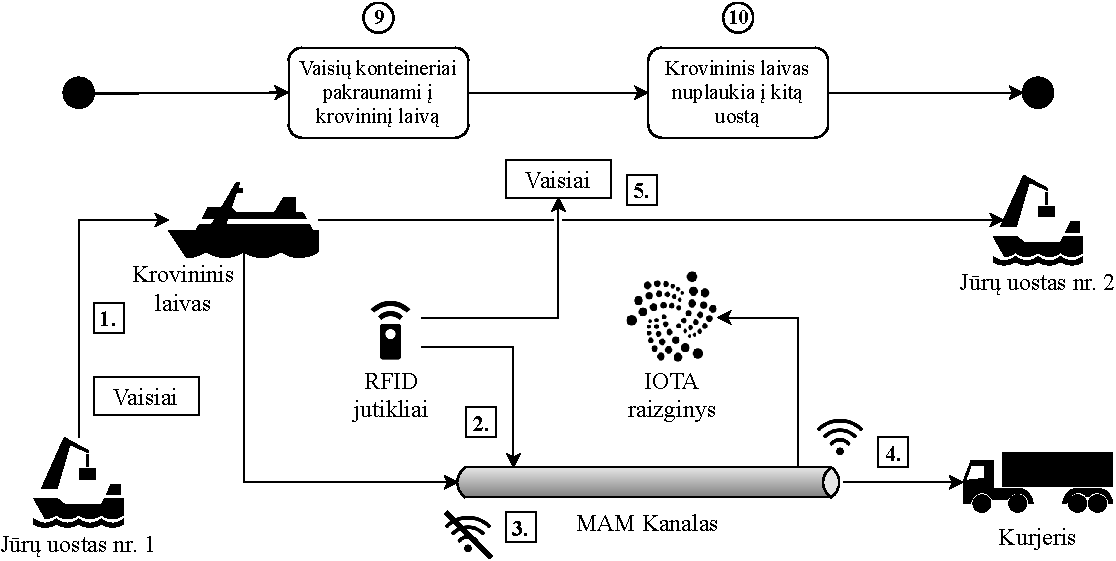
\includegraphics[scale=0.8]{images/iota-usecase-9-10}
    \caption{9 ir 10 etapų papildytas modelis}
    \label{img:16}
\end{figure}



% --------------------------------------------------------------- %
%              3.2.8 VIENUOLIKTAS IR DVYLIKTAS ETAPAI
% --------------------------------------------------------------- %

\subsubsection{Vienuoliktas ir dvyliktas etapai} \label{subsection:uc-11-12}

Vienuoliktojo ir dvyliktojo etapų, \textit{Vaisių konteineriai iškraunami į sunkvežimius} ir \textit{Sunkvežimiai išvežioja vaisius į skirtingas šalis} bendras papildytas modelis (žr.~\ref{img:17} pav.):
\begin{enumerate}
    \item Jūrų uoste nr. 2 iškraunamas konteineris su vaisiais, kurį perima kurjeris.
    \item Kurjeris sukuria MAM kanalą, kurį užprenumeruoja Prekybos centras.
    \item Kurjeris galiausiai pasiekia kitos valstybės muitinę.
\end{enumerate}

\begin{figure}[H]
    \centering
    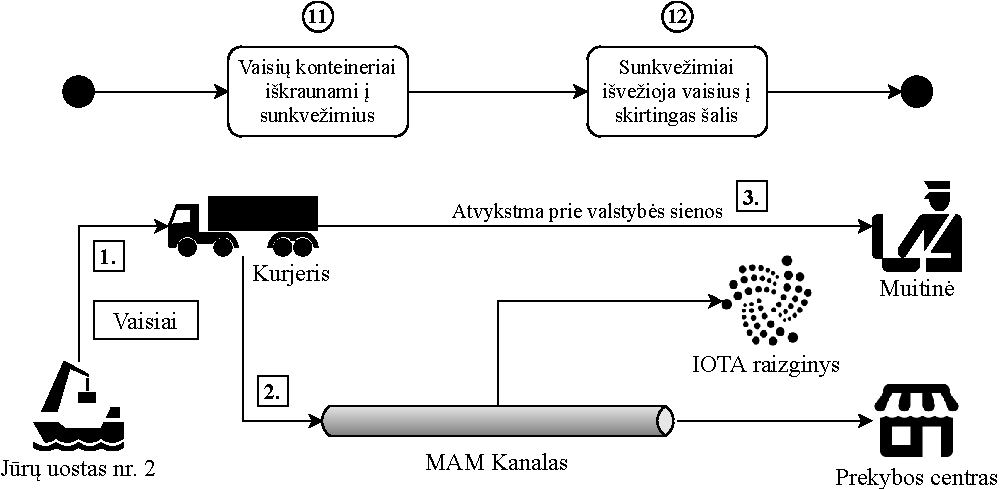
\includegraphics[scale=0.8]{images/iota-usecase-11-12}
    \caption{11 ir 12 etapų papildytas modelis}
    \label{img:17}
\end{figure}



% --------------------------------------------------------------- %
%                       3.2.9 TRYLIKTAS ETAPAS
% --------------------------------------------------------------- %

\subsubsection{Tryliktas etapas} \label{subsection:uc-13}

Tryliktojo etapo papildytas modelis, \textit{Muitinėse patikrinami kroviniai} (žr.~\ref{img:18} pav.):
\begin{enumerate}
    \item Kurjeris perduoda vaisių konteinerį muitinės darbuotojų patikrai.
    \item Muitinės darbuotojai patikrina vaisių kelionės gyvavimo ciklo informaciją IOTA raizginyje. Ši informacija leidžia muitinės darbuotojams lengvai patikrinti svarbią informaciją. Pavyzdžiui, JAV pasienio muitų įstatymas įpareigoja pateikti krovinio pirkėją, pardavėją, gamintoją, kilmės šalį ir kitus duomenis~\cite{customs2018importer}. Visą šią informaciją būtų galima paprastai atsekti ir validuoti IOTA raizginyje, todėl tai galėtų sutaupyti daug laiko. 
    \item Muitinės darbuotojams neradus nieko įtartino, suteikiamas leidimas krovinį įvežti į valstybę. Leidimas taip pat gali būti įrašomas į IOTA raizginį. Vaisius transportuojantis atstovas susimoka muito mokestį (jeigu toks yra taikomas) ir toliau tęsia kelionę.
\end{enumerate}

\begin{figure}[H]
    \centering
    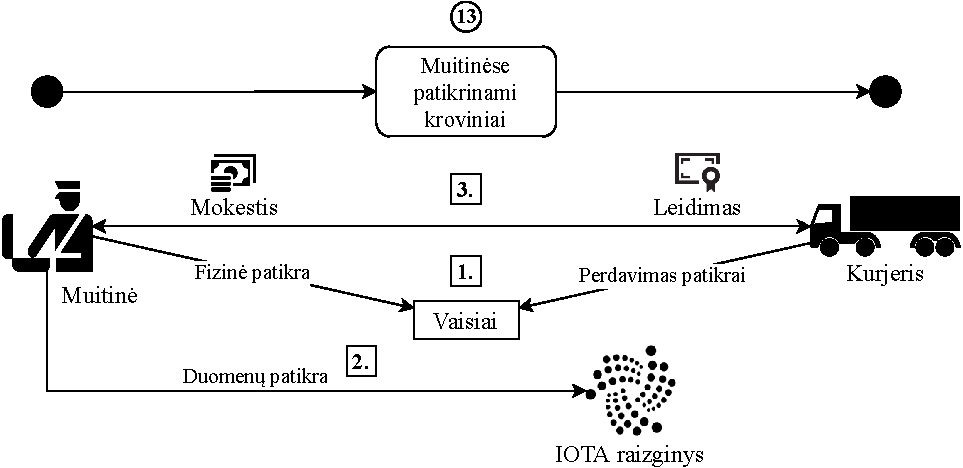
\includegraphics[scale=0.8]{images/iota-usecase-13}
    \caption{13 etapo papildytas modelis}
    \label{img:18}
\end{figure}



% --------------------------------------------------------------- %
%           3.2.10 KETURIOLIKTAS IR PENKIOLIKTAS ETAPAI
% --------------------------------------------------------------- %

\subsubsection{Keturioliktas ir penkioliktas etapai} \label{subsection:uc-14-15}

Keturioliktojo ir penkioliktojo etapų, \textit{Vaisiai išvežiojami į prekybos centrus} ir \textit{Vaisiai parduodami galutiniams pirkėjams} bendras papildytas modelis (žr.~\ref{img:19} pav.):
\begin{enumerate}
    \item Vaisiai transportuojami į prekybos centrą, kuriame šie yra paruošiami pardavimui klientams. Ant vaisių pakuočių prekybos centras pagamina ir užklijuoja specialią informaciją savyje laikantį QR kodo lipduką.
    \item Prekybos centrų klientai nusiperka vaisių pakuotes.
    \item Pirkėjas gali įsitikinti prekybos centro pateikiama informacija, nuskenavęs ant pakuotės esantį QR kodą. Speciali programėlė galėtų leisti peržiūrėti kilmės šalį, vaisių kelionės maršrutą, vaisių auginimo, sandėliavimo ir transportavimo sąlygas, taip pat bet kokią papildomą informaciją, kurią tiekėjai gali atskleisti pirkėjui. Visa ši informacija gaunama iš IOTA raizginyje MAM kanalais bei kitais būdais patalpintos informacijos. Panašiais arba identiškais kodais gali būti žymimi kroviniai visuose tiekimo grandinės etapuose. Pasroviui esantys tiekimo grandinės nariai, prisijungę prie sistemos, galėtų nuskenuoti kodą ir matyti visą jiems aktualią informaciją.
\end{enumerate}

\begin{figure}[H]
    \centering
    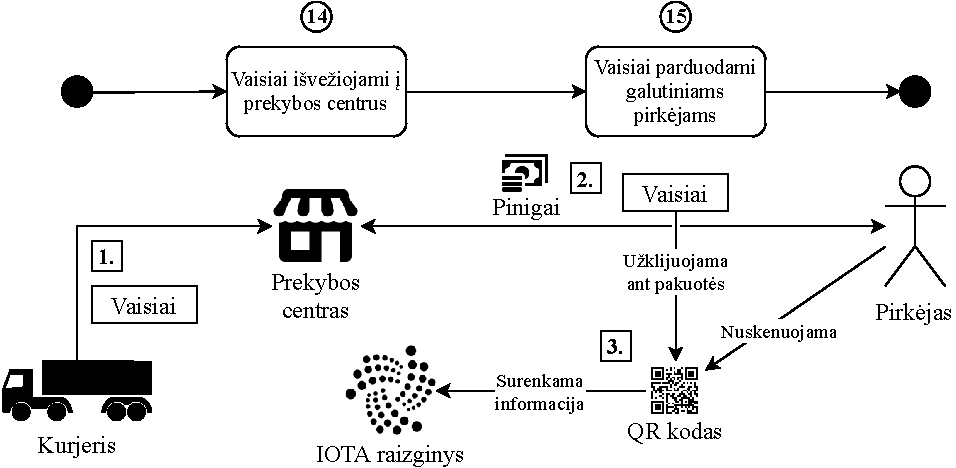
\includegraphics[scale=0.8]{images/iota-usecase-14-15}
    \caption{14 ir 15 etapų papildytas modelis}
    \label{img:19}
\end{figure}



% --------------------------------------------------------------- %
%        3.3 ALTERNATYVŪS IOTA TAIKYMAI TIEKIMO GRANDINĖJE
% --------------------------------------------------------------- %

\subsection{Alternatyvūs IOTA taikymai tiekimo grandinėje} \label{subsection:uc-alt}

3.2. poskyriuose buvo siūlomi IOTA platformos taikymo scenarijai pavyzdinėje tiekimo grandinėje. Tačiau įmanomos įvairios panaudojimo variacijos ir alternatyvos priklausomai nuo situacijos ir poreikio. Šioje dalyje bus nagrinėjamos kelios alternatyvos prieš tai pademonstruotiems panaudojimo atvejo etapų modeliams.

1-12 panaudojimo atvejo etapuose buvo naudojami MAM kanalai. Tačiau šie kanalai buvo sudaromi sukuriant prenumeratos teisę tik pasroviui esančiam tiekimo grandinės dalyviui. Kanalai buvo privatūs, kad informaciją būtų galima siųsti saugiai. Tačiau tiek galutiniai pirkėjai, tiek muitinės, neturėdamos specialaus rakto, gali peržiūrėti tik tą informacinį turinį, kurį pateikia prieš srovę esantis tiekėjas. Vienas iš sprendimo būdų būtų perduoti specialų MAM kanalo prenumeratos raktą visiems pasroviui esantiems tiekimo grandinės dalyviams.

Tačiau tai sukelia papildomų problemų. Skirtingų šalių yra daug: tiesioginiai klientai, netiesioginiai klientai, galutiniai pirkėjai, muitinės ir auditoriai. Visoms šalims reikalinga vis skirtinga informacija. Įmonė nenorėtų, kad konfidenciali informacija, skirta tiesioginiams klientams, pvz. transportavimo tvarkaraščiai arba turimas inventorius, būtų prieinamas galutiniams pirkėjams. Ir atvirkščiai, muitinėms, auditoriams ir galutiniams pirkėjams yra aktuali tik dalis informacijos iš viso srauto.

Naudojant skirtingus MAM kanalus skirstant informaciją tarp tiekimo grandinės šalių ir nustatant skirtingas prieigos teises, galima valdyti informacijos srautus (žr.~\ref{img:20} pav.). Kadangi tiesioginiai klientai keičiasi retai, sukuriamas jam skirtas privatus MAM kanalas. Suvaržytieji kanalai X, Y, ir Z perduoda skirtingus duomenis atitinkamiems prenumeruotojams. Kadangi tiek auditoriai, tiek muitinė, tiek netiesioginiai klientai gali dažnai kisti, yra parenkama suvaržyta kanalų apsauga, leidžianti dinamiškai keisti prenumeruotojus. Viešas kanalas yra skirtas galutiniams pirkėjams, tačiau duomenis gali peržiūrėti bet kas, turintis prieigą prie IOTA raizginio.

\begin{figure}[H]
    \centering
    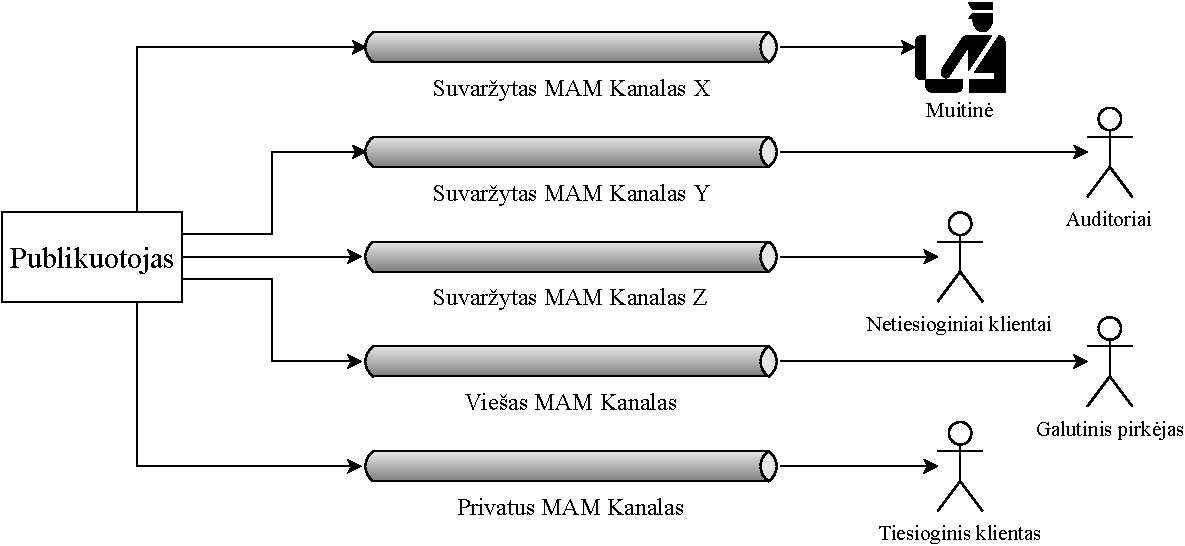
\includegraphics[scale=0.8]{images/mam-channel-flows}
    \caption{Skirtingi MAM kanalų srautai}
    \label{img:20}
\end{figure}

Pavyzdinio panaudojimo atvejo 1, 3, 13-15 etapuose ir bet kuriame kitame etape, kuriame vienas iš žingsnių yra finansinė transakcija, galima naudoti IOTA kaip atsiskaitymo terpę. Tokiam scenarijui pavaizduoti yra tinkamas~\ref{subsection:uc-14-15} poskyryje aprašomas 2 žingsnis. Šiuo atveju galutinis pirkėjas, t.y. prekybos centro klientas perka vaisių pakuotę, už kurią kasoje atsiskaito bankine kortele. Finansine transakcija pasirūpina bankas, o tai, kaip jau buvo minima~\ref{section:dlt} skyriuje, kelia įvairių rizikų.

Tačiau technologijai įsigalėjus klientas galėtų atsiskaityti kriptovaliuta IOTA raizginyje (žr.~\ref{img:21} pav.). Turėdamas savo kriptopiniginę\footnote{Kruptopiniginėje yra laikomos kriptovaliutos. Šiame kontekste kriptopiniginė galėtų būti adresas IOTA raizginyje, kuriame saugomos kriptovaliutos.}, klientas pervestų kriptovaliutą į prekybos centro sąskaitą tiesiogiai ir ši transakcija būtų iškart įrašoma į IOTA raizginį. Tai reiškia, būtų išvengiama tarpininko, šiuo atveju banko. Tokie atsiskaitymai būtų galimi ir didesniais mastais, pavyzdžiui, milijoniniai finansiniai sandoriai tarp verslo šalių. Žinoma, tam reikėtų visuotinio technologijos ir kriptovaliutos pripažinimo ir nusistovėjimo, nes šiuo metu jos kaina labai svyruoja\footnote{Duomenys iš: \href{https://coinmarketcap.com}{https://coinmarketcap.com} [žiūrėta 2019-05-17].}.

\begin{figure}[H]
    \centering
    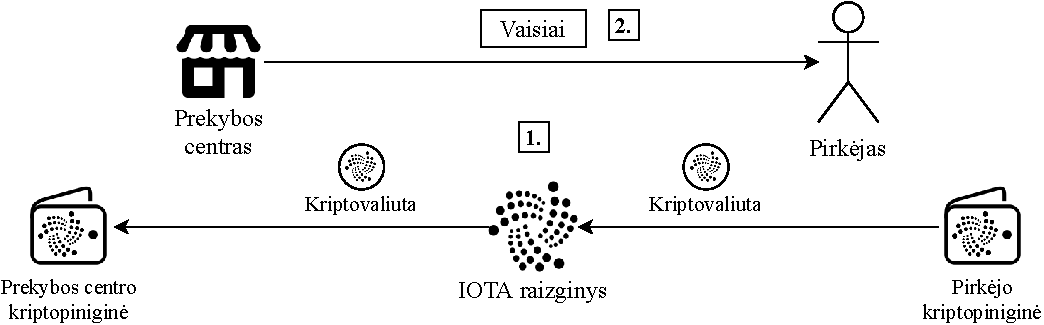
\includegraphics[scale=0.75]{images/tangle-financial-transaction}
    \caption{Finansinė transakcija IOTA raizginyje}
    \label{img:21}
\end{figure}

Pavyzdinio panaudojimo atvejo 2 etape svarbų vaidmenį vaidina orakulai, įrašydami savo duomenis į IOTA raizginį. Tai leidžia patikrinti, ar ūkininko pateikiami duomenys atitinka realybę. Tačiau 2 etapo 3 žingsnį galima praplėsti naudojant orakulus ir išmaniuosius kontraktus (žr.~\ref{img:22} pav.): 
\begin{enumerate}
    \item Geografiniame regione, kuriame ūkininkas augina vaisius, galėtų būti įsikūrę daugybė orakulų, kurie turėtų savo temperatūros matavimo prietaisus. Šiais prietaisais jie pamatuotų temperatūrą arba kitus rodiklius.
    \item Kiekvienas orakulas perduotų savo duomenis išmaniajam kontraktui. Šioje vietoje įmanomas sandorio sudarymas tarp išmaniojo kontrakto savininko ir orakulų. Sandoris įpareigotų orakulus tiekti informaciją išmaniajam kontraktui už tam tikrą kriptovaliutos mokestį.
    \item Išmanusis kontraktas surinktų visų orakulų duomenis ir juos visus perduotų išoriniam skaičiavimų įrenginiui. Atlikus skaičiavimus įrenginys grąžintų gautą skaičiavimų rezultatą išmaniajam kontraktui.
    \item Gautus galutinius skaičiavimus ir kitą informaciją išmanusis kontraktas perduotų MAM kanalu, kurį yra užsiprenumeravęs supirkėjas.
\end{enumerate}

\begin{figure}[H]
    \centering
    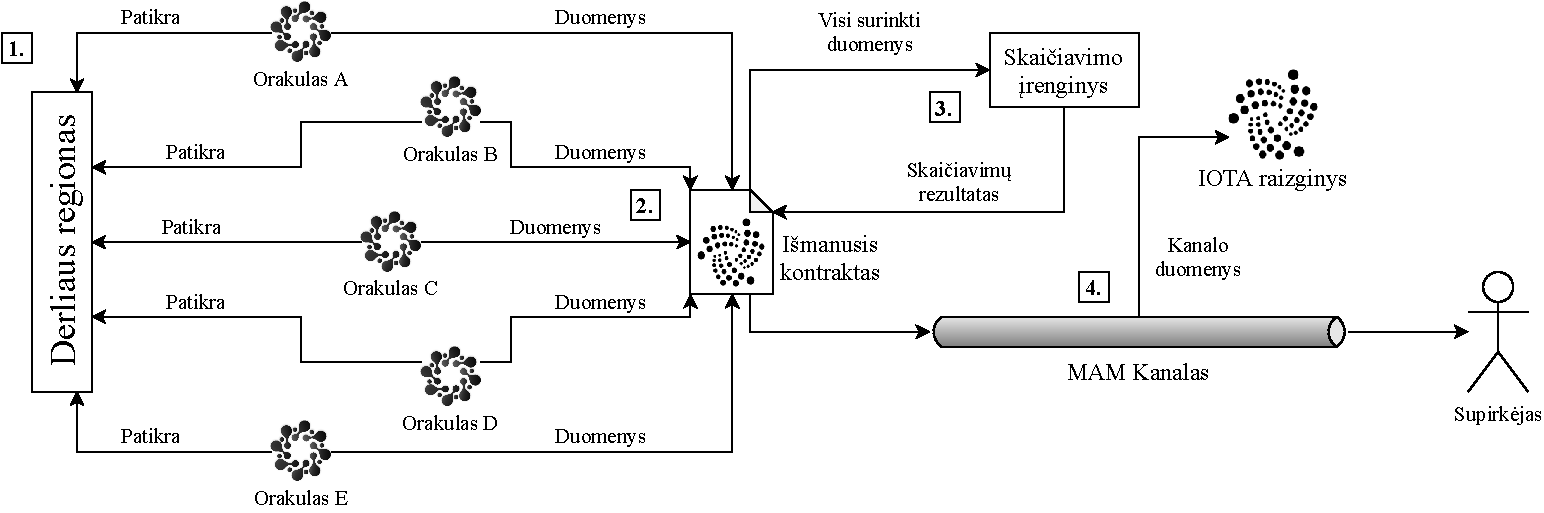
\includegraphics[scale=0.63]{images/tangle-smart-contract}
    \caption{Išmaniojo kontrakto ir orakulų bendradarbiavimas}
    \label{img:22}
\end{figure}



% --------------------------------------------------------------- %
%               3.4 BŪSIMOS SISTEMOS UŽDUOTYS IR VEIKLOS
% --------------------------------------------------------------- %

\subsection{Potencialios sistemos užduotys ir veiklos} \label{subsection:uc-system}

Norint įgyvendinti IT sistemą, įgalinančią IOTA panaudojimą panašioje į tiekimo grandinę, pavaizduotą priede~\ref{appendix:1}, svarbu apsibrėžti sistemoje dalyvaujančias šalis, jų užduotis ir veiklas sistemoje. Remiantis 12-22 paveikslėliuose pavaizduotų siūlomų sprendimų modeliais, buvo surinktos esminės tiekimo grandinės veiklos, kurias galima įgyvendinti potencialioje sistemoje. Taip pat atrinkti visi tiekimo grandinėje esantys dalyviai. Gautas rezultatas pavaizduotas matricoje (žr.~\ref{tab:2} lentelė). 

\begin{table}[h]
\centering
\caption{Skirtingų šalių dalyvavimo tiekimo grandinės procesuose matrica}
\label{tab:2}
\begin{tabular}{|l|l|l|l|l|l|l|l|l|l|l|}
\hline
\textbf{Veikla} & \multicolumn{1}{c|}{\textbf{A}} & \multicolumn{1}{c|}{\textbf{B}} & \textbf{C} & \textbf{D} & \textbf{E} & \textbf{F} & \textbf{G} & \textbf{H} & \textbf{I} & \textbf{J} \\ \hline
Sudaryti sandorį & + & + & + & + & + & + &  & + & + &  \\ \hline
Patikrinti dokumento teisėtumą & + & + & + & + & + & + & + & + & + &  \\ \hline
Sukurti MAM kanalą & + & + & + & + & + & + & + &  & + &  \\ \hline
Prenumeruoti MAM kanalą &  & + & + & + & + & + & + & + & + & + \\ \hline
Siųsti kriptovaliutą &  & + & + &  & + &  &  &  & + & + \\ \hline
Gauti kriptovaliutą & + & + & + & + & + & + &  & + & + & + \\ \hline
Perduoti duomenis išmaniajam kontraktui &  &  &  &  &  & + &  &  &  &  \\ \hline
Generuoti QR kodą &  & + & + & + & + &  & + & + &  &  \\ \hline
Nuskaityti QR kodą &  &  & + & + & + &  & + & + &  & + \\ \hline
\end{tabular}
\end{table}

Lentelė reikalauja specialaus paaiškinimo. Kiekvienas stulpelio antraštės simbolis A-J reiškia vis skirtingą tiekimo grandinėje dalyvaujančią rolę. A – sėklų tiekėjas, B – ūkininkas, C – vaisių supirkėjas, D – kurjeris, E – prekybos centras, F – orakulas, G – muitininkas, H – jūrų uostas, I – išmaniojo kontrakto savininkas, J – galutinis pirkėjas. Langeliai su „+“ simboliu reiškia, kad atitinkama tiekimo grandinės šalis dalyvauja tam tikrame procese.

Autorius pastebi, kad potenciali sistema gali turėti daugybę kitų funkcionalumų, tokių kaip registracija, prisijungimas, istorijos peržiūra ir t.t. Tačiau šiame darbe nagrinėjamos pagrindinės bazinės sistemos veiklos, tiesiogiai susijusios su IOTA taikymo tiekimo grandinėje pavyzdžiais. 

Dar vienas svarbus reikalavimas, kurį turi įgyvendinti sistema – tai nuolatinė prieiga prie IOTA raizginio. Tai yra būtina tam, kad sistemos ir raizginio duomenys visada būtų sinchronizuoti ir būtų remiamasi naujausia raizginio informacija. Tam užtikrinti reikalingas interneto ryšys. Nors, kaip jau minėta~\ref{subsection:dag-offline} ir~\ref{subsection:uc-9-10} poskyriuose, tam tikrais atvejais sistema būtų galima naudotis ir neturint interneto prieigos.

Kiekviena ~\ref{tab:2} lentelėje pažymėta veikla turi būti prieinama atitinkamoms šalims per sistemos naudotojo sąsają naudotojui prisijungus. Tai reiškia, kad turi būti sukuriamos skirtingos sistemos būsenos priklausomai nuo to, koks naudotojas yra prisijungęs. 

Tam, kad skaitytojui būtų paprasčiau įvertinti, ką ir kaip potenciali sistema turėtų atlikti, darbo autorius siūlo supaprastintus sistemos veiklų scenarijus, kuriems buvo nubraižytos panaudos atvejų ir veiklų UML diagramos. Visos diagramos buvo parengtos remiantis matricos duomenimis (žr.~\ref{tab:2} lentelė) naudojant \textit{draw.io} naršyklės įrankį. 

Priede~\ref{appendix:2} ir priede~\ref{appendix:3} pavaizduotos sistemos užduočių diagramos, parodančios sistemos rolių (angl. \textit{Actors}) galimas užduotis. Prieduose nr. 4-8 pavaizduotos veiklų diagramos, parodančios kaip ir kokiais scenarijais įvairios rolės ir sistema bendrauja tarpusavyje.
% ----------------------------------
% --------------------------------------------------------------- %
%                            REZULTATAI                           
% --------------------------------------------------------------- %

\sectionnonum{Rezultatai}

Darbo rezultatai:
\begin{enumerate}
    \item Sumodeliuotas pavyzdinis tiekimo grandinės atvejis, sudarytas iš 15 diskrečių etapų;
    \item Pasiūlyti IOTA taikymo pavyzdinėje tiekimo grandinėje sprendimų scenarijai kiekvienam etapui bei alternatyvos daliai jų;
    \item Pateikti potencialios sistemos, įgyvendinančios IOTA pritaikymą tiekimo grandinėse, veikėjai, jų užduotys ir pagrindiniai veiklos scenarijai.
\end{enumerate}
\sectionnonum{Išvados}

Išvados:
\begin{enumerate}
    \item išvada
\end{enumerate}

%Išvadų skyriuje daromi nagrinėtų problemų sprendimo metodų palyginimai, siūlomos rekomendacijos, akcentuojamos naujovės. Išvados pateikiamos sunumeruoto (gali būti hierarchinis) sąrašo pavidalu. Darbo išvados turi atitikti darbo tikslą.

Tolimesnės tyrinėjimo kryptys:
% --------------------------------------------------------------- %
%                           BIBLIOGRAFIJA                           
% --------------------------------------------------------------- %

\printbibliography[heading=bibintoc]
% --------------------------------------------------------------- %
%                              SĄVOKOS                           
% --------------------------------------------------------------- %

\sectionnonum{Sąvokų apibrėžimai}

\noindent \textbf{51\% ataka} - vienas iš išskirstyto transakcijų žurnalo atakos būdų, kuomet kenkėjas bando turėti daugiau nei 50\% viso tinklo pajėgumų ir šitaip jį užvaldyti.

\noindent \textbf{Atlikto darbo konsensuso algoritmas} - konsensuso algoritmas, paremtas dalyvavimu tinkle atliekant skaičiavimus.

\noindent \textbf{Bitcoin} - pirmoji blokų grandinės principu paremta platforma, pristatyta 2008 metais.

\noindent \textbf{Blokas} - blokų grandinių architektūrinis vienetas ir duomenų struktūra, laikanti savyje kitus duomenis.

\noindent \textbf{Blokų grandinė} - Viena iš išskirstytų transakcijų technologijos atmainų, kuri savyje laiko duomenis, tarpusavyje sujungtus į nuoseklių blokų seką.

\noindent \textbf{CRM} - ryšių su klientais valdymo sistema, padedanti organizuoti ir valdyti visos įmonės darbą, nukreiptą į esamų ir potencialių klientų poreikių patenkinimą. 

\noindent \textbf{Decentralizuota programėlė} - programinis kodas, vykdomas išskirstytose sistemose.

\noindent \textbf{Dvigubo išleidimo problema} - potenciali spraga skaitmeninių pinigų sistemoje, kuomet tas pats piniginis vienetas gali būti išleistas ir priklausyti daugiau nei vienam asmeniui tuo pačiu metu.

\noindent \textbf{Ekonominis klasteris} - grupė IOTA tinklo narių, esančių tame pačiame regione.

\noindent \textbf{ERP} - programinė įranga, skirta kompiuterizuoti įmonės valdymą apjungiant duomenis ir procesus joje.

\noindent \textbf{Ethereum} - blokų grandinės principu paremta platforma, pirmą kartą pristatyta 2014 metais.

\noindent \textbf{GAS limitas} - Ethereum platformos vienetas, skirtas nusakyti, maksimalų GAS, kurį transakcijos kūrėjas yra linkęs išleisti už transakcijos patvirtinimą tinkle.

\noindent \textbf{GDPR reglamentas} - Europos Parlamento ir Europos Tarybos priimtas visoje ES tiesiogiai taikomas teisės aktas, įgyvendinantis asmens duomenų apsaugos reformą.

\noindent \textbf{IOTA} - orientuotų grafų be ciklų principu paremta platforma, pirmą kartą pristatyta 2015 metais.

\noindent \textbf{IOTA raizginys} - IOTA tinklo apibūdinimas.

\noindent \textbf{Išmanusis kontraktas} - programinis kodas, automatiškai vykdantis komandas pagal prieš tai aprašytas taisykles.

\noindent \textbf{Išskirstyto transakcijų žurnalo technologija} - duomenų bazė, kuria konsensuso būdu dalinasi ir operuoja skirtingi naudotojai tinkle.

\noindent \textbf{Kasėjas} - asmuo, atliekantis skaičiavimus blokų grandinėse su tikslu sukurti bloką ir už tai gauti kriptovaliutos atlygį.

\noindent \textbf{Konsensuso algoritmas} - protokolas, kuris pasirūpina, kad visi tinklo nariai sinchronizuotųsi tarpusavyje ir prieitų bendrą sutarimą.

\noindent \textbf{Kriptopiniginė} – skaitmeninė piniginė, skirta kriptovaliutų siuntimui, gavimui ir laikymui.

\noindent \textbf{Kriptovaliuta} - skaitmeninis turtas, naudojamas išskirstytų transakcijų žurnalų transakcijose.

\noindent \textbf{Maišos reikšmė} - tam tikro ilgio skaitinė reikšmė, skirta identifikuoti unikalius duomenis.

\noindent \textbf{MAM kanalas} - specialus darinys IOTA tinkle, leidžiantis sukurti duomenų srautą, kurį gali prenumeruoti kiti asmenys tinkle.

\noindent \textbf{Markov Chain Monte Carlo algoritmas} - algoritmas, skirtas pasirinkti ir patvirtinti IOTA tinkle esančias viršūnes.

\noindent \textbf{Maskuotieji nustatytos tapatybės pranešimai} - biblioteka, užšifruojanti, iššifruojanti ir nustatanti tapatybę duomenų, kuriuos yra norima publikuoti į IOTA raizginį.

\noindent \textbf{Orakulas} - IOTA tinklo tarpininkas su išoriniu pasauliu.

\noindent \textbf{Orientuotas grafas be ciklų} - grafas, kurio visos briaunos turi kryptį ir savyje neturintis ciklų.

\noindent \textbf{Panaudos atvejo diagrama} - UML diagrama, apibūdinanti, ką projektuojama sistema gali atlikti, kartu aprašydama ir išorinius sistemos veikėjus. 

\noindent \textbf{Qubic protokolas} - protokolas, veikiantis kaip atskiras IOTA sluoksnis, įgalinantis išmaniuosius kontraktus, orakulus ir išskirstytus skaičiavimus.

\noindent \textbf{Raizginio viršūnė} - IOTA raizginio transakcija, kurios nėra patvirtinusi jokia kita transakcija.

\noindent \textbf{RFID prietaisai} - priemonės, skirtos radijo dažnio bangų pagalba siųsti žinutes.

\noindent \textbf{Stiprinanti transakcija} - speciali transakcija IOTA tinkle, kuriama naudotojo savo paties transakcijų patvirtinimo tinkle tikimybei padidinti.

\noindent \textbf{TEU standartas} - standartinis vienetas, paremtas ISO 20 pėdų ilgio konteineriu ir naudojamas kaip statistinė eismo srauto ar mato priemonė.

\noindent \textbf{Tiekimo grandinė} - organizacijų, procesų, finansų, informacijos ir kitų esybių visuma, dalyvaujanti produkto gyvavimo cikle nuo pradinio tiekėjo iki galutinio kliento.

\noindent \textbf{Transakcijos kaupiamasis svoris} - IOTA transakcijos atributas, nusakantis šios transakcijos ir visų kitų transakcijų, tiesiogiai arba netiesiogiai patvirtinančių šią transakciją, svorių suma.

\noindent \textbf{Transakcijos per sekundę} - dydis, skirtas nusakyti, kiek transakcijų arba įrašų atsiduria transakcijų žurnale per sekundę.

\noindent \textbf{Transakcijos svoris} - IOTA transakcijos atributas, nusakantis, kiek tinklo naudotojas įdėjo pastangų sukurdamas transakciją.

\noindent \textbf{Transakcijos taškai} - IOTA transakcijos atributas, nusakantis visų tiesiogiai arba netiesiogiai šios transakcijos patvirtintų kitų transakcijų ir kartu šios transakcijos svorių sumą.

\noindent \textbf{Turimos įtakos konsensuso algoritmas} - konsensuso algoritmas, paremtas turimos įtakos tinkle, pavyzdžiu kriptovaliuta, disponavimu.

\noindent \textbf{Veiklų UML diagrama} - UML diagrama, aprašanti konkretaus scenarijaus vykdomus veiksmus.

\noindent \textbf{Viršūnių parinkimo algoritmas} - algoritmas, skirtas IOTA tinklo dalyviams atsirinkti transakcijas, kurios bus patvirtintos.

\noindent \textbf{Winternitz vienkartinė parašo panaudojimo schema} - kvantiniams kompiuteriams atspari schema, skirta generuoti viešus raktus IOTA tinkle.
\sectionnonum{Santrumpos}
TEU - 
CRM
ERP

\appendix  

\section{Įprasta tiekimo grandinė (Vertikaliai)}
\begin{figure}[H]
    \centering
    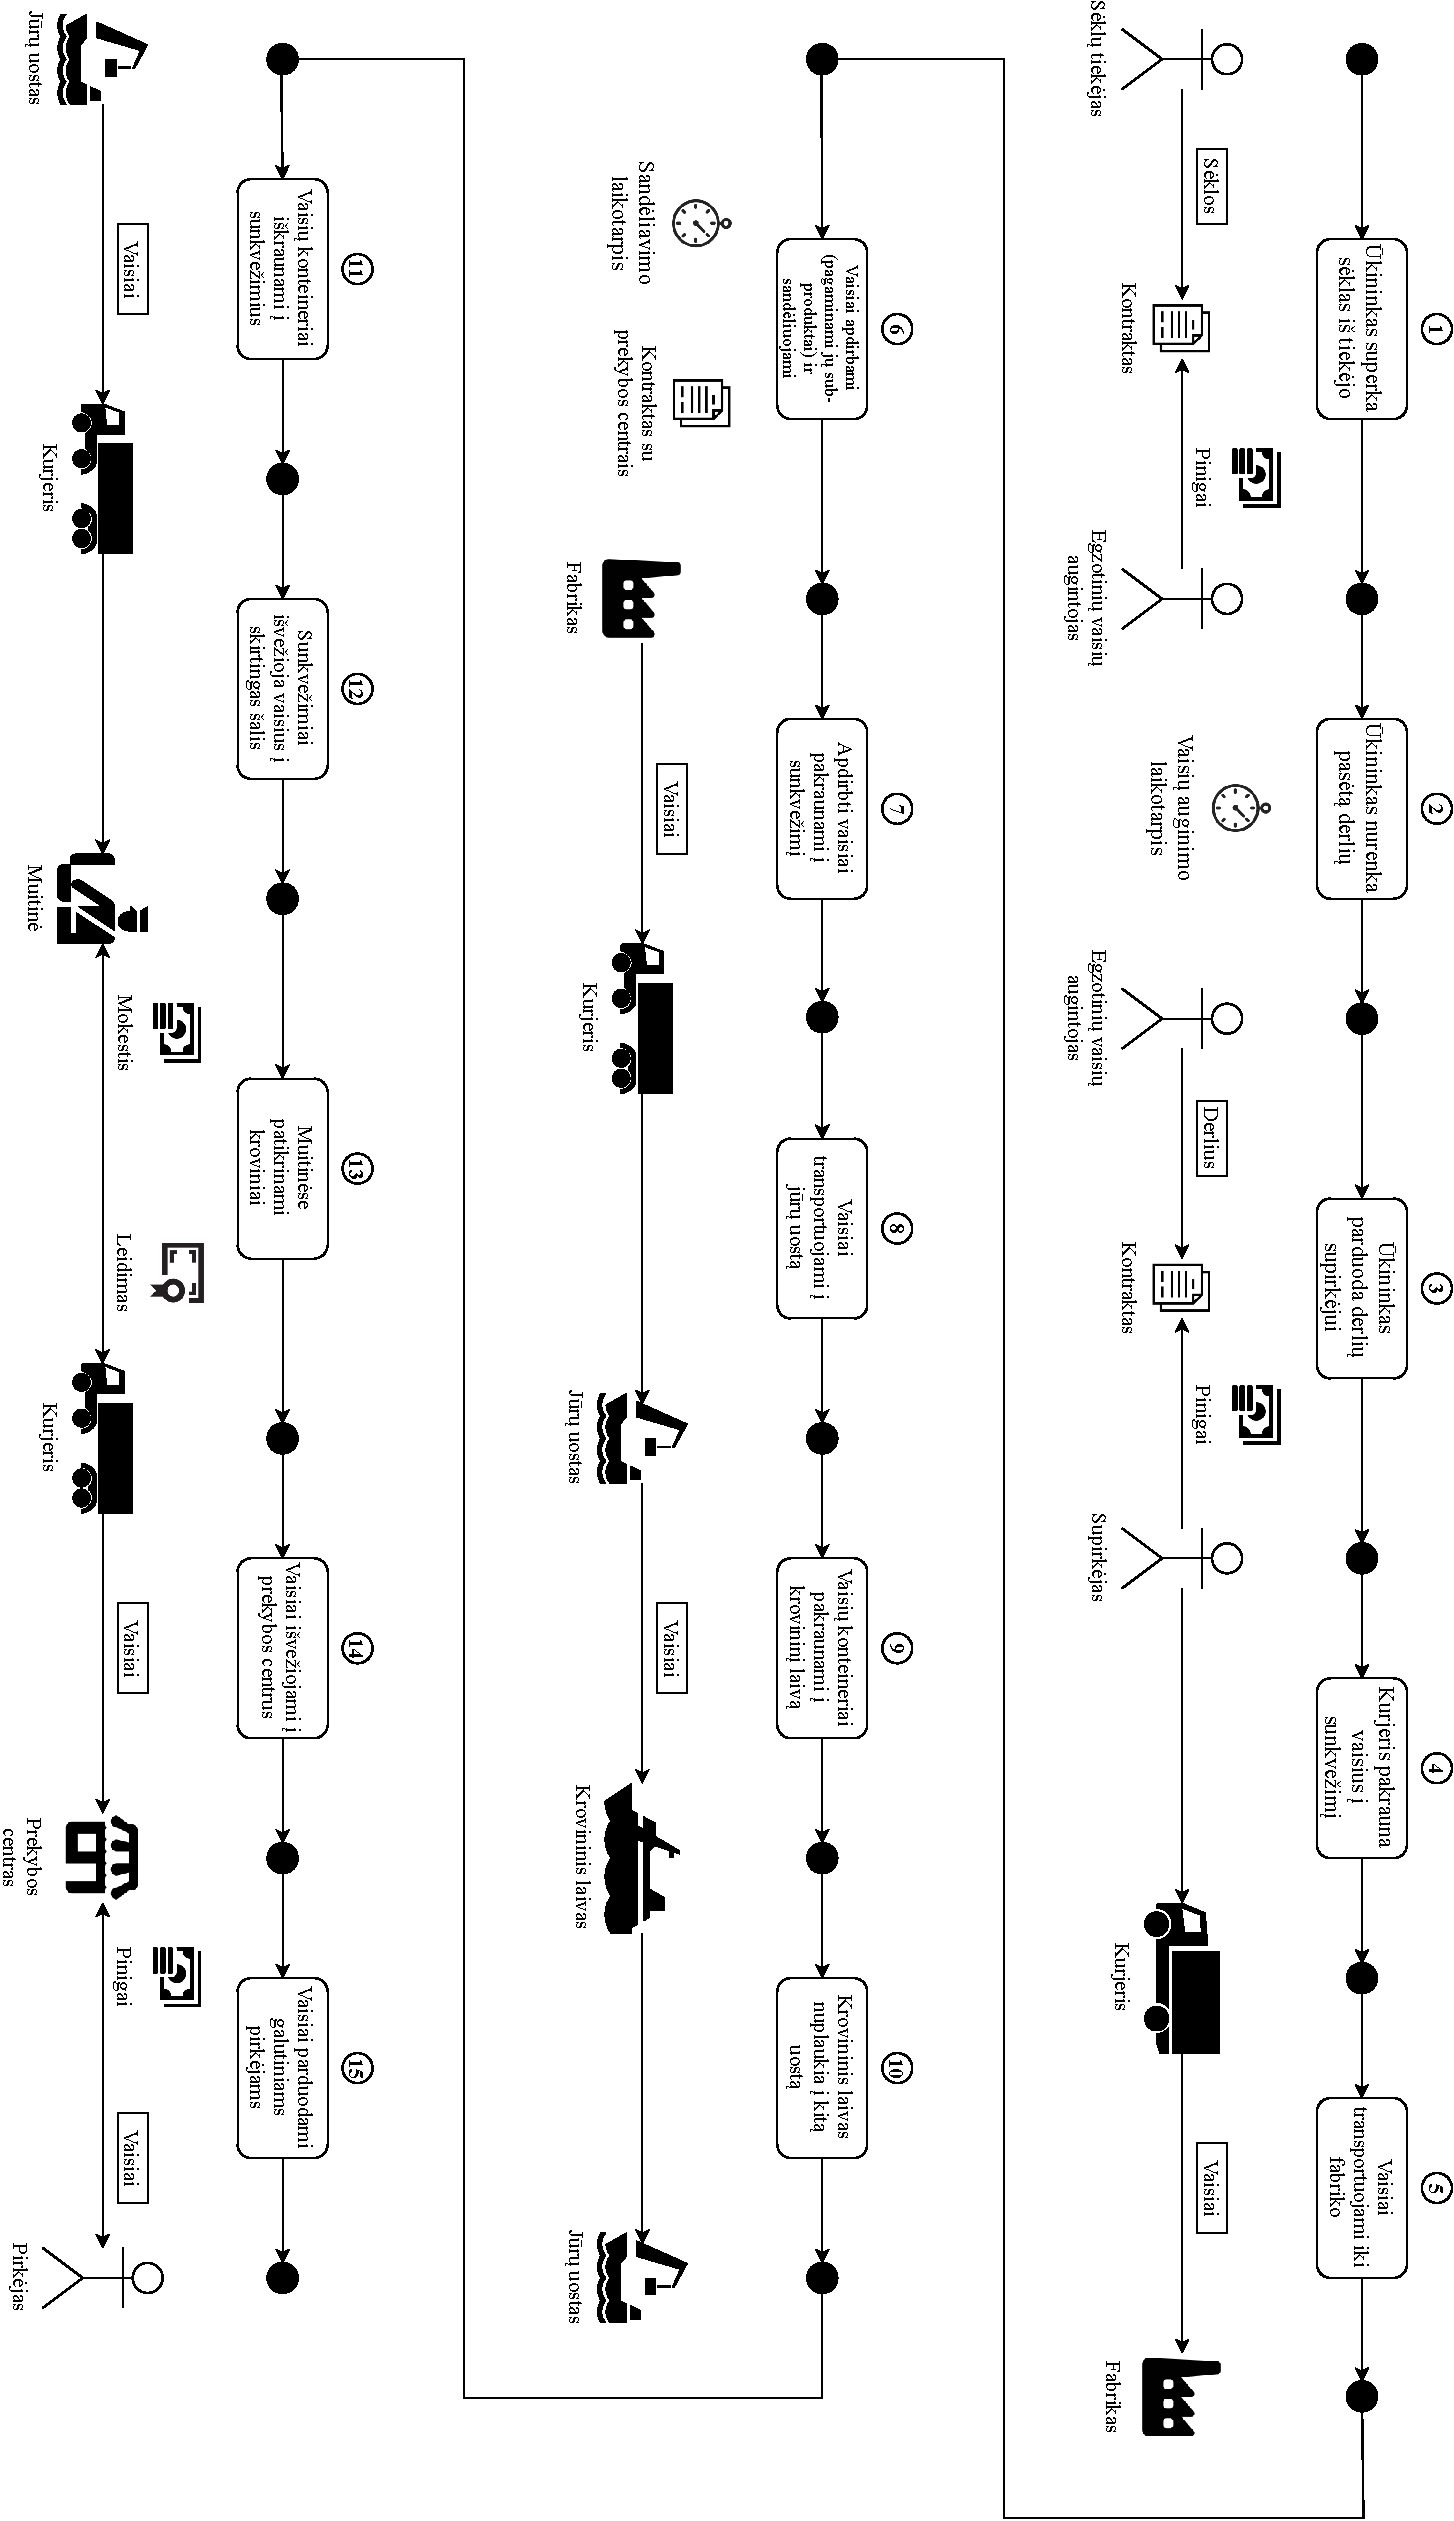
\includegraphics[scale=0.52]{images/supply-chain-vertical}
    \caption{Įprasta tiekimo grandinė (Horizontaliai)}
\end{figure}

\section{Įprasta tiekimo grandinė (Horizontaliai)}
\begin{figure}[H]
    \centering
    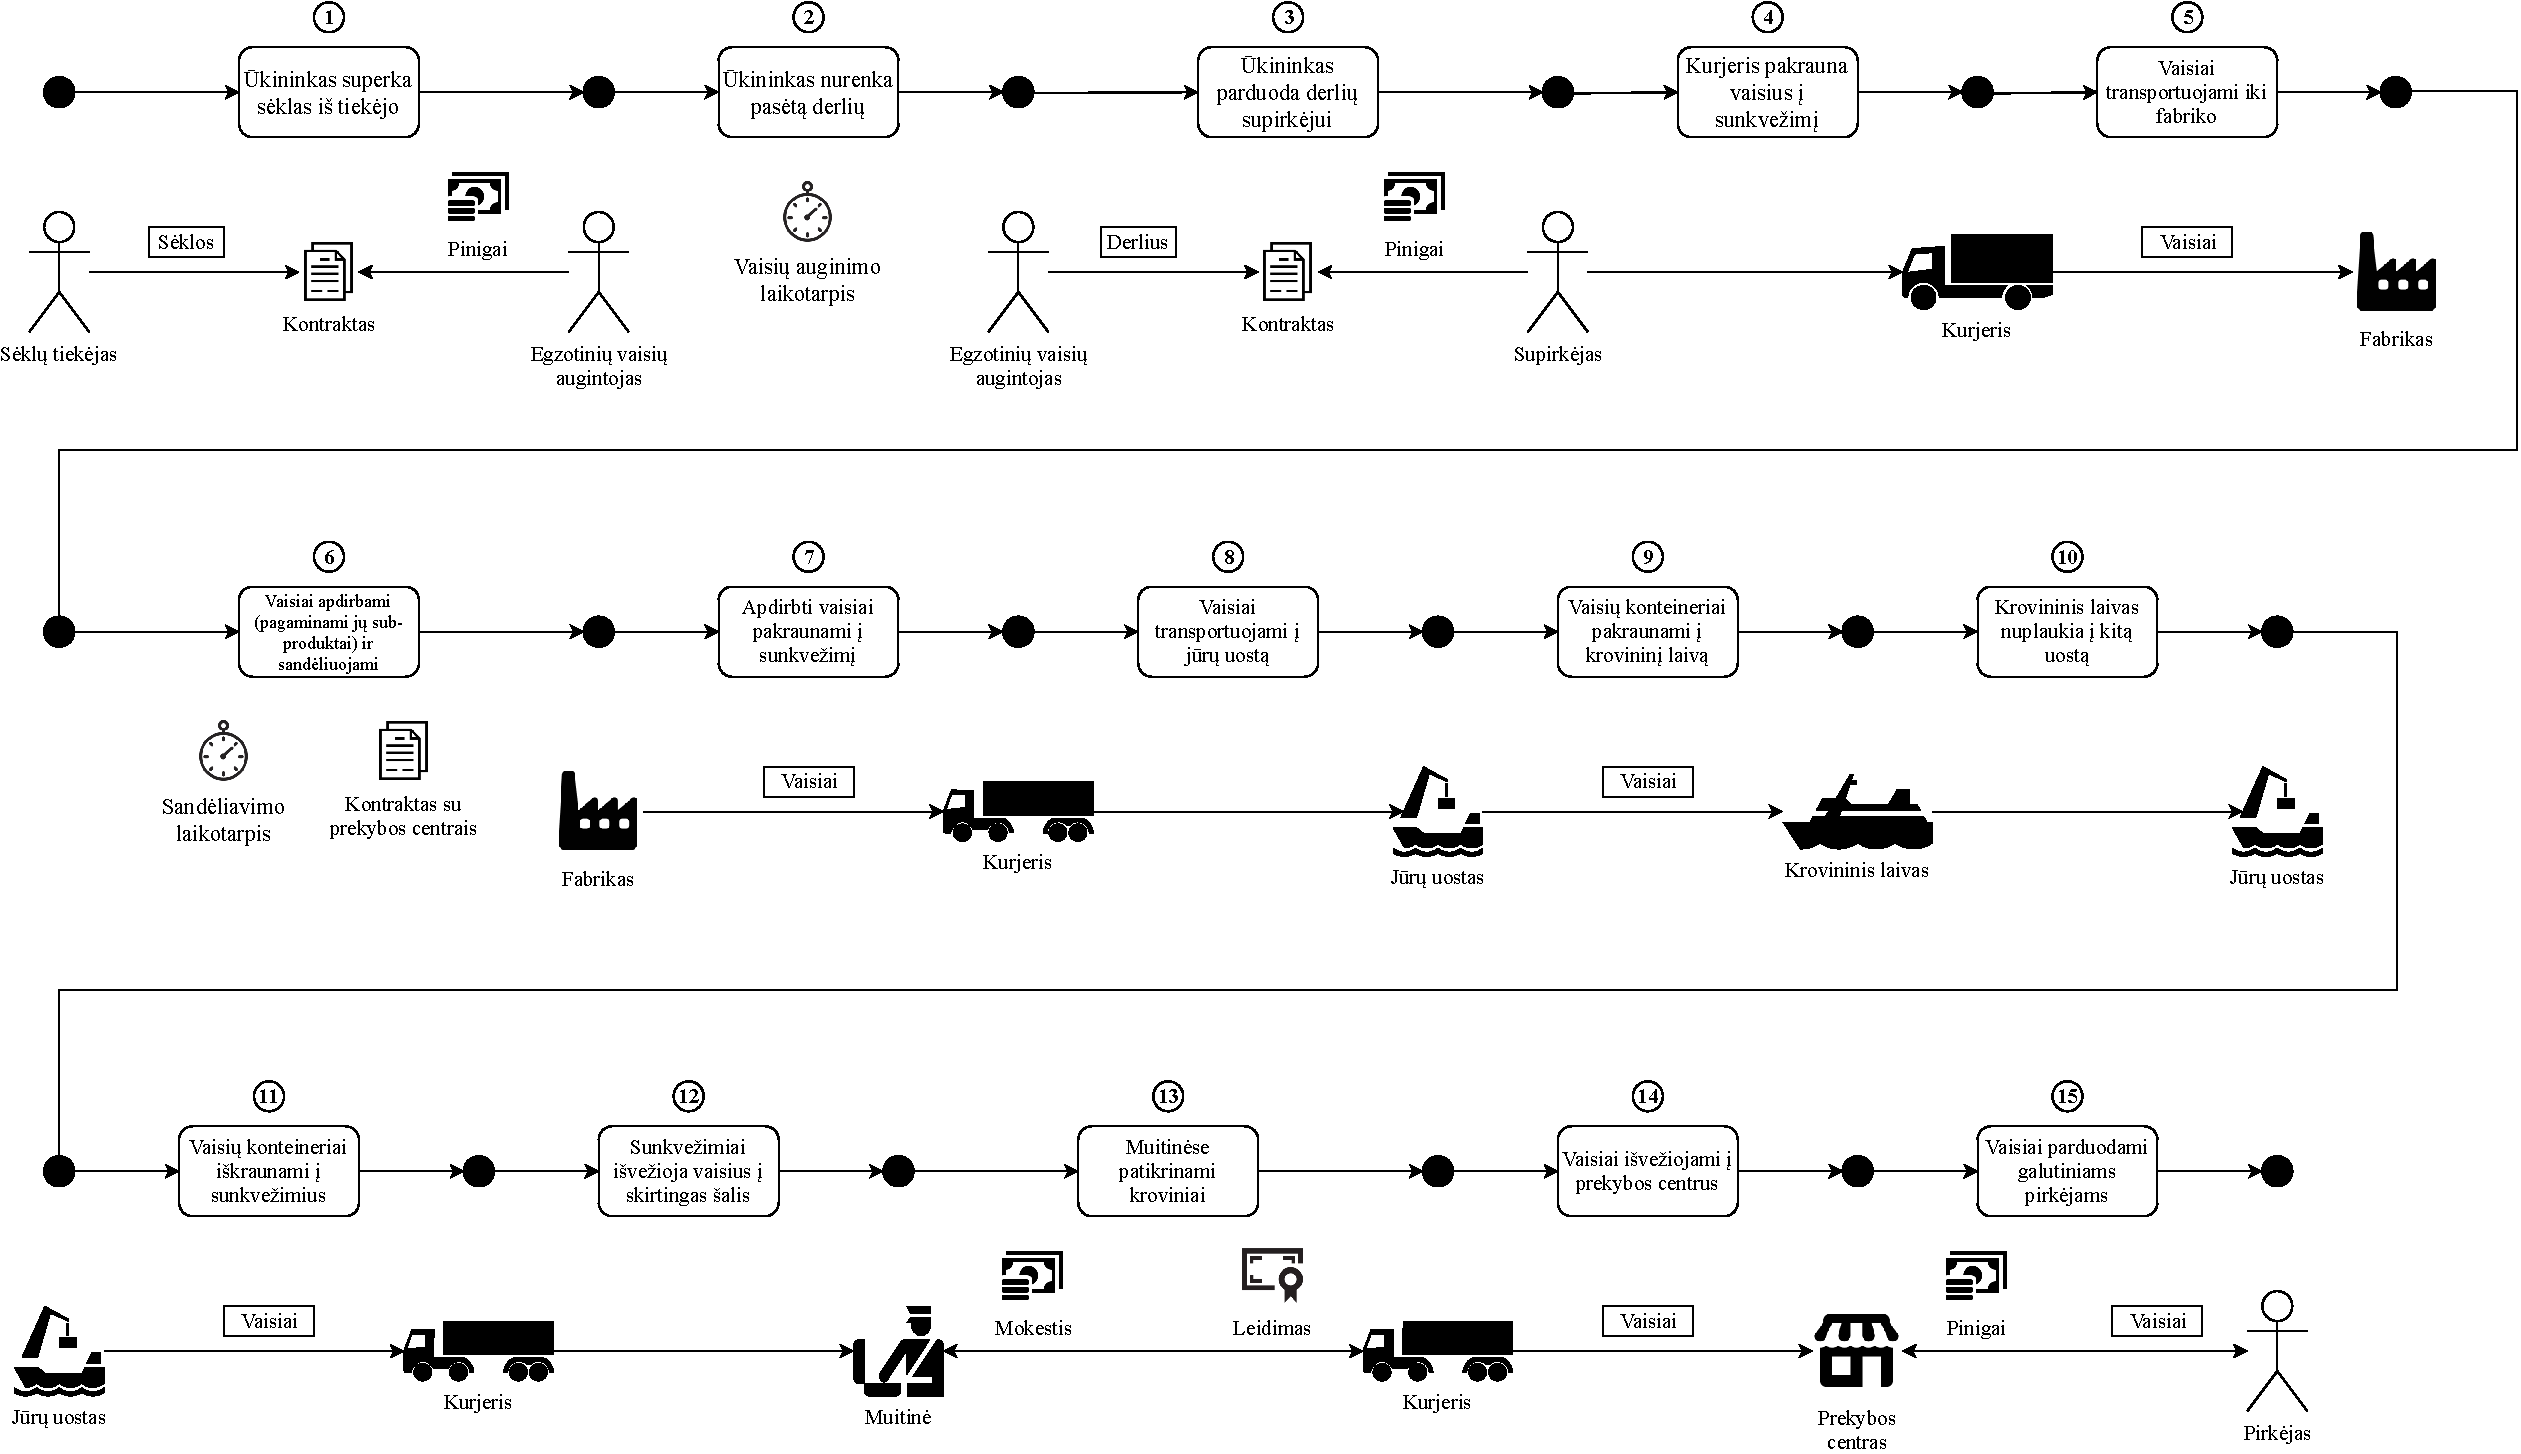
\includegraphics[scale=0.4]{images/supply-chain-horizontal}
    \caption{Įprasta tiekimo grandinė}
\end{figure}

% Prieduose gali būti pateikiama pagalbinė, ypač darbo autoriaus savarankiškai
% parengta, medžiaga. Savarankiški priedai gali būti pateikiami ir
% kompaktiniame diske. Priedai taip pat numeruojami ir vadinami. Darbo tekstas
% su priedais susiejamas nuorodomis.

\end{document}